\documentclass{ieeeaccess}
\usepackage{cite}
\usepackage{amsmath,amssymb,amsfonts}
\usepackage{graphicx}
\usepackage{textcomp}
\usepackage{booktabs}
\usepackage{float}
\usepackage{placeins}
\usepackage{algorithm}
\usepackage{algpseudocode}
\usepackage{makecell}
\usepackage{url}

\usepackage{bm}
\makeatletter
\AtBeginDocument{\DeclareMathVersion{bold}
\SetSymbolFont{operators}{bold}{T1}{times}{b}{n}
\SetSymbolFont{NewLetters}{bold}{T1}{times}{b}{it}
\SetMathAlphabet{\mathrm}{bold}{T1}{times}{b}{n}
\SetMathAlphabet{\mathit}{bold}{T1}{times}{b}{it}
\SetMathAlphabet{\mathbf}{bold}{T1}{times}{b}{n}
\SetMathAlphabet{\mathtt}{bold}{OT1}{pcr}{b}{n}
\SetSymbolFont{symbols}{bold}{OMS}{cmsy}{b}{n}
\renewcommand\boldmath{\@nomath\boldmath\mathversion{bold}}}
\makeatother

\def\BibTeX{{\rm B\kern-.05em{\sc i\kern-.025em b}\kern-.08em
    T\kern-.1667em\lower.7ex\hbox{E}\kern-.125emX}}

\renewcommand{\thetable}{\Roman{table}}

%Your document starts from here ___________________________________________________
\begin{document}
\history{Date of publication xxxx 00, 0000, date of current version xxxx 00, 0000.}
\doi{10.1109/ACCESS.2024.0429000}

\title{Mitigating Class Imbalance in Pump-and-Dump Detection: A Comparative Analysis of Imbalance-Aware Algorithms}
\author{\uppercase{M. Mironov}\authorrefmark{1},
\uppercase{D. Bogutsky}\authorrefmark{2}, and P. \uppercase{Lukianchenko}\authorrefmark{3}}

\address[1]{National Research University Higher School of Economics, Faculty of Computer Science, Laboratory of AI in Mathematical Finance (e-mail: mvmironov@hse.ru)}

\address[2]{National Research University Higher School of Economics, Faculty of Computer Science, Laboratory of AI in Mathematical Finance (e-mail: dbogucki@hse.ru)}

\address[3]{National Research University Higher School of Economics, Faculty of Computer Science, Laboratory of AI in Mathematical Finance (e-mail: plukyanchenko@hse.ru)}

\tfootnote{
This work was supported by the grant for research centers in the field of AI provided by the Ministry of Economic Development of the Russian Federation in accordance with the agreement 000000C313925P4E0002 and the agreement with HSE University № 139-15-2025-009}

\markboth
{Mironov, Bogutsky, Lukianchenko \headeretal: Mitigating Class Imbalance in Pump-and-Dump Detection}
{Mironov, Bogutsky, Lukianchenko \headeretal: Mitigating Class Imbalance in Pump-and-Dump Detection}

\corresp{Corresponding author: D. Bogutsky (e-mail: dbogucki@hse.ru).}

\begin{abstract}
The cryptocurrency market has been subject to various forms of exploitation, with pump-and-dump schemes being a persistent problem that can lead to significant price volatility and financial losses. Previous studies have focused on predicting attack targets using machine learning approaches; however, these methods are often compromised by class imbalance and biases inherent in historical data. To address this limitation, we present an empirical framework for comparing manipulation-target prediction methods.
We employ two-step bias-minimizing data normalization techniques to mitigate the effects of class imbalance and temporal heterogeneity. We compare established class-weighted, oversampling, and ranking approaches using a common event-level protocol.
Validation Top@k\%AUC selects CatBoost ($0.653$). It attains test Top@1 $0.188$, Top@10 $0.500$, and Top@k\%AUC $0.689$ on 80 events. L2 logistic regression has the highest descriptive test AUC ($0.710$); paired resampling does not establish a significant AUC difference between these two models.
We validate the results using resampling and evaluate the validation-selected model in portfolio backtests incorporating transaction costs and price impact.
\end{abstract}

\begin{keywords}
Classification, Imbalanced Datasets, Learning to rank, Machine Learning, Market Manipulation, Market Microstructure, Portfolio strategy
\end{keywords}

\titlepgskip=-21pt

\maketitle

\section{Introduction}
\label{sec:introduction}
\subsection{What are Pumps and Dumps}

\PARstart{P}{ump-and-dump} schemes (P\&Ds) are a type of fraudulent activity that involves artificially inflating the price of a cryptocurrency through coordinated buying efforts, followed by a rapid selling to unsuspecting investors. This phenomenon is often characterized by an abrupt and significant increase in trading volume, followed by a subsequent decline in price as the original buyers liquidate their positions.

These schemes typically involve experienced traders and market manipulators who orchestrate the operation through various channels, including online forums and social media platforms such as Telegram channels. The manipulation is designed to create a false sense of urgency and scarcity, which attracts inexperienced investors who may be unaware of the true nature of the event.

A typical pump-and-dump scenario can be observed in Fig.~\ref{fig:pump_and_dump_example}, which shows a clear example of this phenomenon. The figure illustrates price movements associated with a specific token VIB traded against BTC on Binance exchange, highlighting the abrupt spike in trading activity following the announcement of the token's release. This sudden increase in volume is often followed by a rapid decline in price as insiders sell their positions to new buyers.

\begin{figure}[h!]
    \centering
    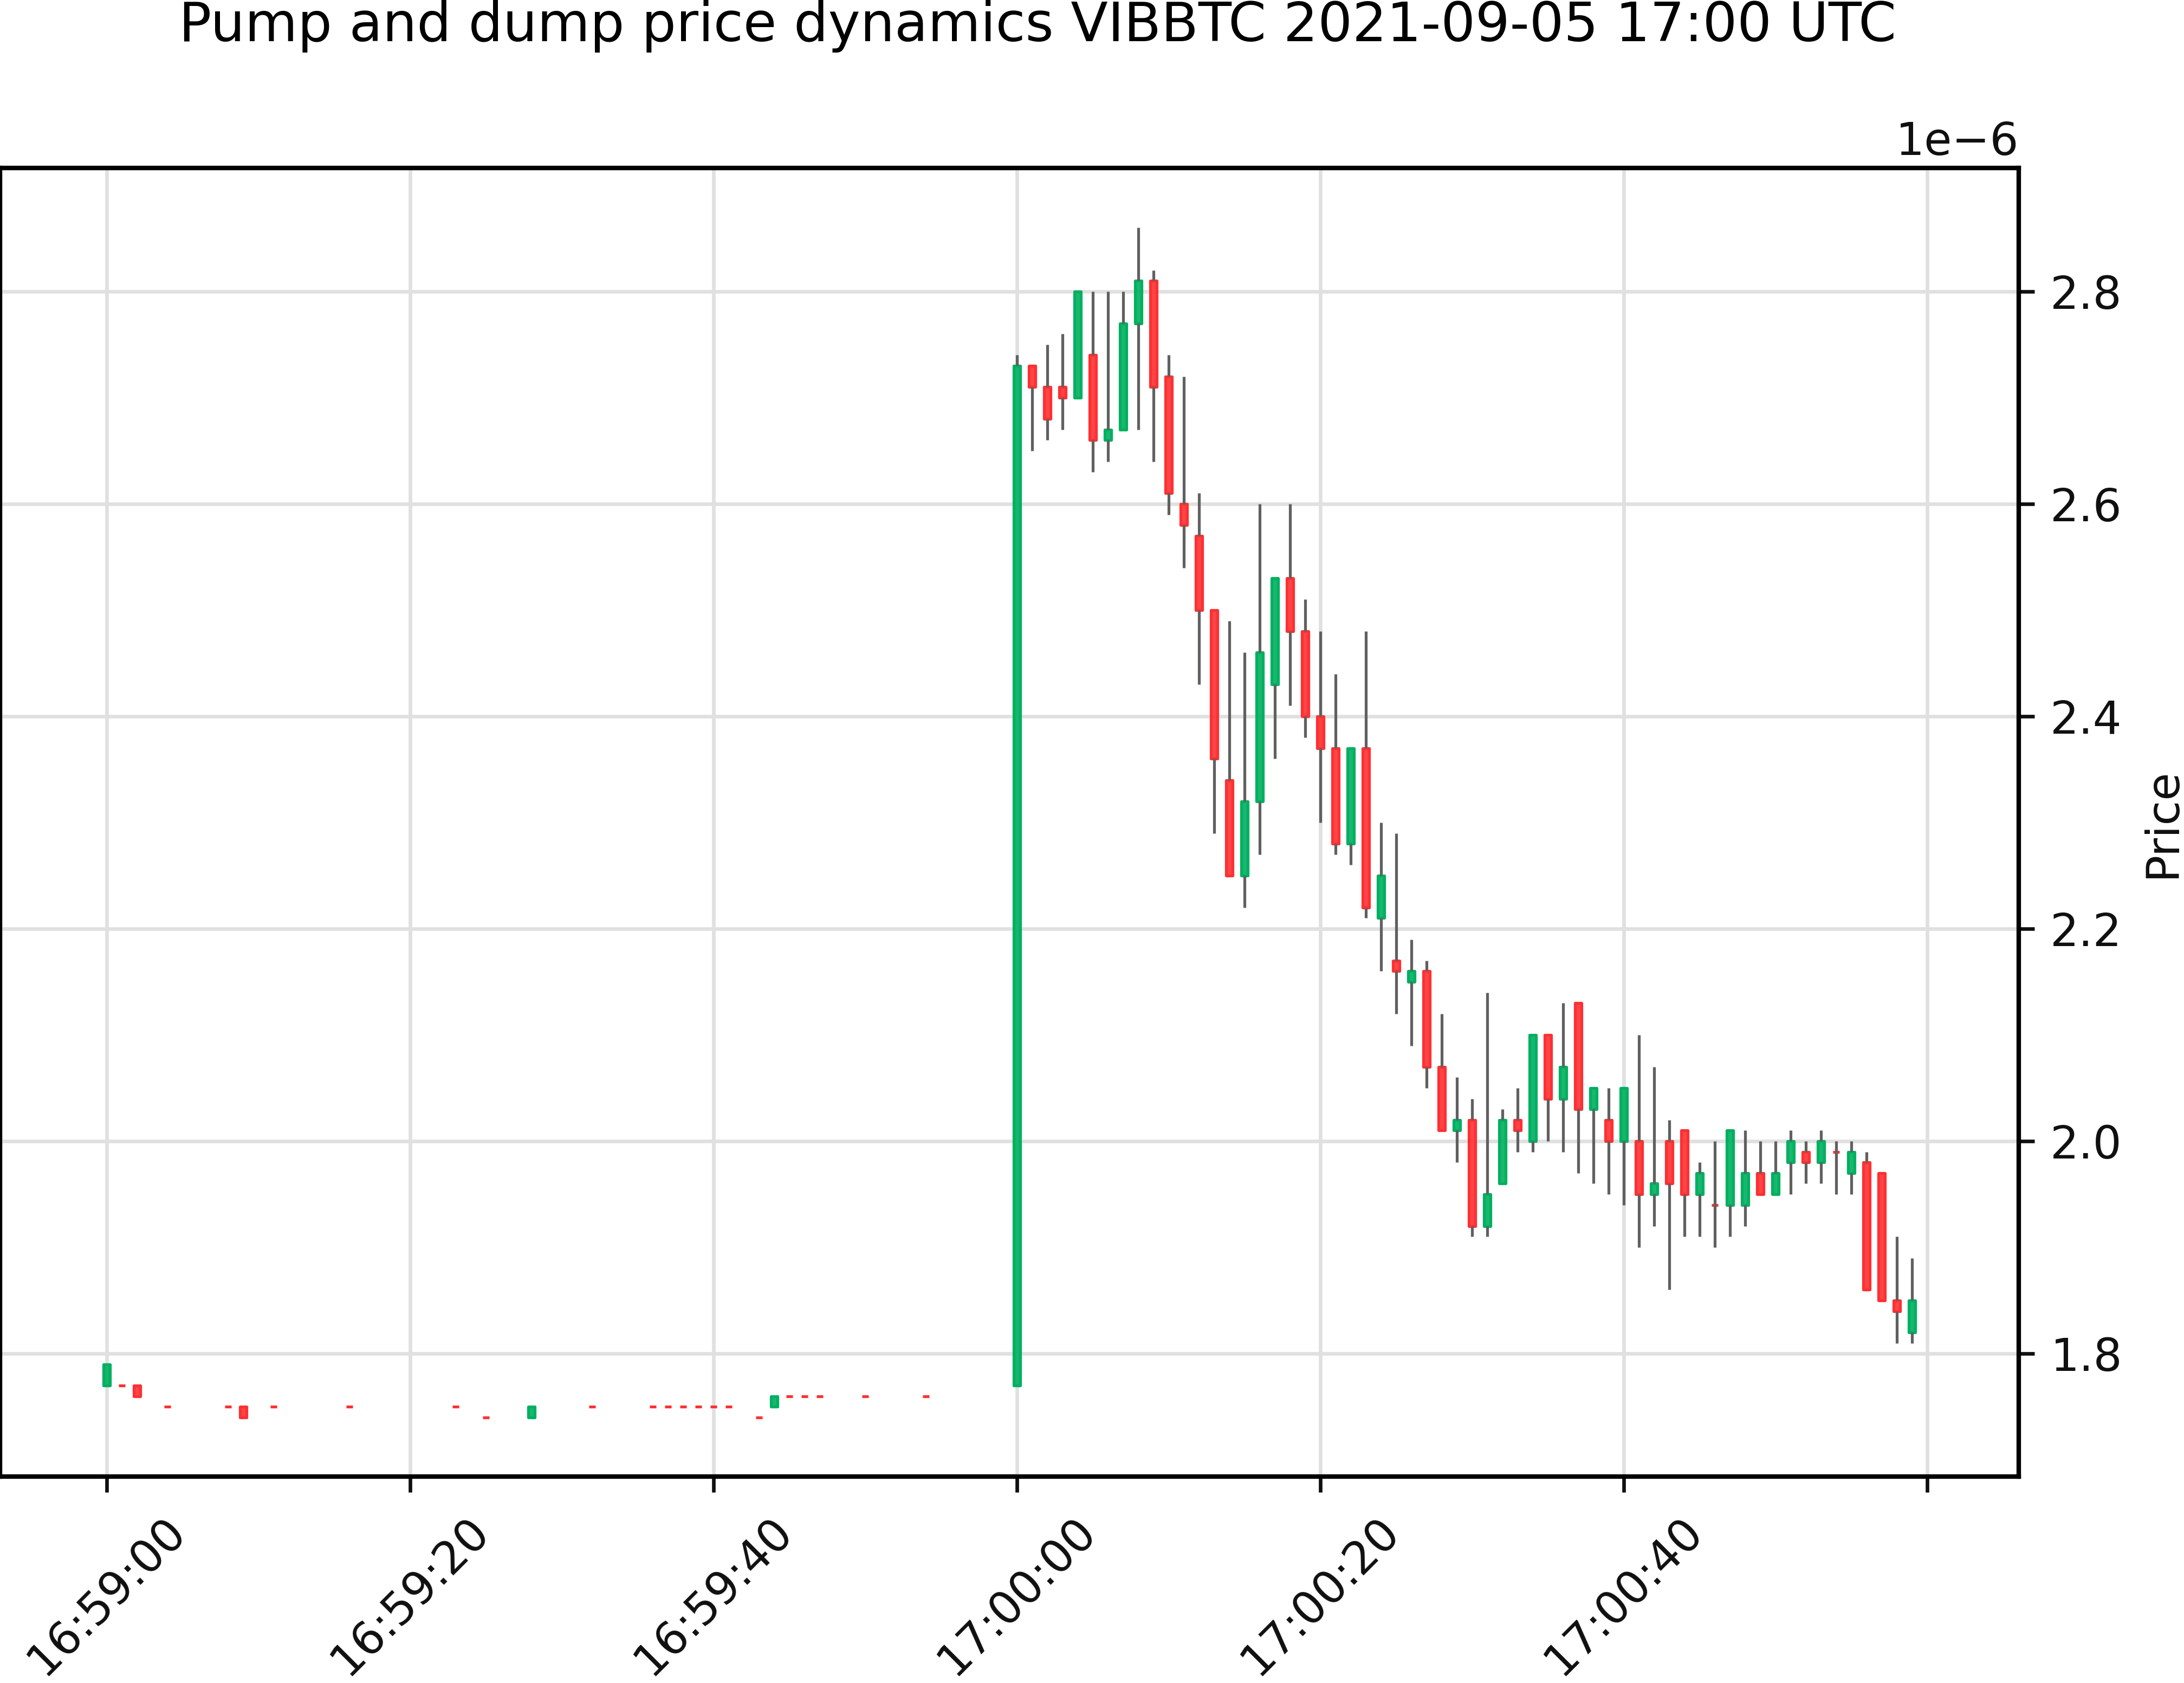
\includegraphics[scale=0.5]{images/pump_and_dump_example.png}
    \caption{VIBBTC pump and dump manipulation carried out on Binance}
    \label{fig:pump_and_dump_example}
\end{figure}

\subsection{Related Work}

The phenomenon of pump-and-dump schemes has been extensively studied in the context of cryptocurrencies, with research efforts spanning multiple approaches and methodologies.

One of the pioneering studies on this topic was \cite{kamps_moon_2018}, which introduced a comprehensive framework for understanding pump-and-dump operations. The authors highlighted the targeting of small market cap cryptocurrencies due to their lower trading volumes, utilizing data from 5 prominent crypto exchanges: Binance, Bittrex, Kraken, Kucoin, and Lbank. Their analysis covered pumps history of 1.5 years, with price and volume data being used as the primary sources. Subsequent research efforts have focused on leveraging machine learning (ML) algorithms to enhance P\&D detection accuracy. La Morgia et al.'s work \cite{la_morgia_pump_2020}, \cite{la2023doge} employed random forest algorithms, achieving improved results compared to traditional rule-based approaches. The authors in \cite{chadalapaka_crypto_2022} further increased the effectiveness of La Morgia's work by incorporating Deep Neural Networks (LSTMs and Transformers) as anomaly detection algorithms.
More recently, in \cite{econometrics11030022} the authors built on these findings by studying a similar pump dataset between 2021 and 2022. They developed an innovative approach that employed resampling methods, such as SMOTE, combined with price and volume features and random forest classification to detect pump events 1 hour in advance.

In addition to pump detection, other research has focused on predicting the maximum price move during known pump events. Nghiem et al. \cite{nghiem_2021} used market data and social sentiment with deep neural networks (LSTMs and CNNs) and achieved promising results. However, their analysis highlighted a potential limitation of using sentiment signals: historical bias may be introduced due to the lack of precise snapshots of historical social data.

A relevant example of work addressing the problem of predicting price manipulation targets is the study \cite{pd_anatomy}. This research proposed an approach using random forest algorithms to identify potential pump and dump schemes among listed tokens. The authors analyzed a dataset of 180 pump events from the Cryptopia exchange, incorporating features such as price and volume data, global market capitalization data from Coinmarketcap, and token ratings by exchange. To enhance model robustness, the study employed filtering techniques to exclude pumps with suspicious announcement times that deviated significantly from full hours. Moreover, the authors validated their classification model through backtesting a portfolio strategy based on predicted pump targets. However, it is worth noting that the employed trading strategy relied on unrealistic assumptions, such as guaranteed profits of half the maximum price move during the pump and zero losses for false positive predictions.

A related study was conducted in \cite{hu2023sequence}, where authors enhanced their approach by incorporating channel embeddings into their model. They also utilized standard price and volume metrics, as well as external data sources such as market capitalization and social media information (e.g., Twitter followers, Reddit subscribers, Alexa rank). The analysis was performed on a dataset comprising 445 pump announcement events. However, due to the presence of duplicate pump events across multiple channels, the actual number of unique pump events studied is smaller than expected. Furthermore, the use of social data from different sources raises concerns about historical bias, as these metrics may have changed after the fact, potentially affecting the accuracy of the results.

Regarding market manipulation in a broad sense, several papers have also been published recently, for example \cite{cong_washtrading_2023}, which studied the manipulation of trading volumes, also known as wash trading.

With the increasing popularity of ML applications in finance, in recent years we have seen many articles on predictions using the market microstructure, for example \cite{albers_frag_2022} and \cite{ntakaris_midprice_2022}. Promising results have also been published with applications of ranking models to finance \cite{poh_ltr}.  Taking into account the rich accumulated experience in related areas, we aim to complement existing work with new factors based on the market microstructure.

In the broader ML literature, several families of techniques have been proposed for handling class imbalance beyond resampling, and each maps imperfectly onto the P\&D target-prediction problem. Cost-sensitive learning~\cite{elkan2001cost} re-weights the loss so that misclassifying the minority class is more expensive; it does so without perturbing the feature space, which, as we show empirically in Section~\ref{section:results}, can be an advantage when features are already cross-sectionally normalized. Focal loss~\cite{lin2017focal}, originally proposed for dense object detection, down-weights easy examples and concentrates the gradient on hard, informative ones; it has since been adopted for imbalanced tabular classification, but remains most effective when combined with deep models and large minority classes, conditions that do not apply to our 290 positive training events. Synthetic oversampling methods such as SMOTE~\cite{chawla2002smote} have known pathologies in high-dimensional settings~\cite{blagus2013smote}, which is consistent with our results in Section~\ref{section:results}.

Anomaly detection provides a complementary formulation that does not require balanced training data. Isolation Forest~\cite{liu2008isolation} and related one-class approaches have been applied to fraud and market-abuse detection when positive examples are essentially unavailable. In our setting, however, positive examples \emph{are} available (at least in limited numbers) and the task is explicitly \emph{cross-sectional}: we do not ask ``is this observation anomalous in isolation?'' but rather ``which asset in this cross-section is the most likely manipulation target?''. This ranking-within-cross-section structure makes the problem closer to learning-to-rank than to unsupervised anomaly detection, and motivates the imbalance-aware ranking metric (Top@k\%AUC) that we adopt as the training target throughout this paper. Our comparison combines cross-sectional panel normalization, microstructure features, and an imbalance-aware ranking objective for the one-positive-versus-many-negatives event structure.


This paper builds upon previous work in \cite{pd_anatomy} and \cite{hu2023sequence}, which focused on predicting manipulation targets among traded assets. We identify several critical limitations in data preparation that limit model reliability and evaluate established remedies under a common event-level protocol. Specifically, we combine microstructure-based features using insights from areas of market prediction \cite{albers_frag_2022}, \cite{ntakaris_midprice_2022} and wash trading detection \cite{cong_washtrading_2023}. Moreover, we explore the use of boosted trees, as implemented in CatBoost \cite{catboost}, which has been shown to outperform other algorithms on tabular data (e.g., \cite{grinsztajn_2022}), and we compare their performance to the random forest model introduced in \cite{random_forest_2001}.

To further improve the classification models' performance, we also perform a cross-sectional normalization method for panel data. Moreover, we formulate a specialized metric tailored to optimize the classification model for highly unbalanced datasets, which was used for model training and validation.

The contribution is empirical integration and comparison, rather than a new learning algorithm: event-level ranking evaluation, common microstructure predictors, and explicit execution sensitivity on a documented Binance BTC-pair sample. Leakage prevention requires auditing preprocessing as well as chronological splits~\cite{kapoor2023leakage,cerqueira2020evaluation}; recent imbalance-learning surveys likewise distinguish data-level resampling from algorithm-level weighting~\cite{chen2024imbalance}. In cryptocurrency markets, quoted fees alone need not capture trading costs: changes in spreads and depth can offset fee reductions~\cite{galati2024fees}. These distinctions motivate the separation of predictive evaluation and simulated execution below.

Table~\ref{table:comparison_prior_work} summarizes the key methodological differences between our framework and the most closely related prior studies.

\begin{table*}[!t]
    \centering
    \small
    \renewcommand{\arraystretch}{1.3}
    \setlength{\tabcolsep}{5pt}
    \caption{Comparison of the proposed framework with closely related prior work on P\&D target prediction}
    \begin{tabular}{p{2.8cm}p{2.2cm}p{2cm}p{2.2cm}p{2.5cm}p{2.5cm}}
        \toprule
        \textbf{Study} & \textbf{Exchange} & \textbf{\# Events} & \textbf{Model} & \textbf{Imbalance Handling} & \textbf{Backtesting} \\
        \midrule
        Xu \& Livshits~\cite{pd_anatomy} & Cryptopia & 180 & Random forest & None & Unrealistic assumptions \\
        Hu et al.~\cite{hu2023sequence} & Multiple & 445 & Seq. model + channel embed. & None & None \\
        Fantazzini \& Xiao~\cite{econometrics11030022} & Binance & Varies & Random forest & SMOTE & None \\
        La~Morgia et al.~\cite{la_morgia_pump_2020} & Multiple & 1111 & Random forest & None & None \\
        \textbf{Ours} & Binance & 473 & CatBoost, LR, RF, Ranker & Cross-sectional norm., Top@k\%AUC opt., class weighting & Impact-aware execution \\
        \bottomrule
    \end{tabular}
    \label{table:comparison_prior_work}
\end{table*}

\section{Data Collection and Preprocessing}

\subsection{Labeled P\&Ds data}
\label{section:pump_and_dump_data}

The released event list contains 498 unique announced P\&D targets on Binance spot BTC pairs between January~3, 2018 and August~14, 2022. Each record supplies the target pair, exchange, and UTC announcement timestamp. These announcement labels are the fixed input to the empirical pipeline; no event is retained or discarded according to its subsequent return.

\paragraph{Channel identification.}
We identified eight candidate Telegram channels through a two-step procedure. First, we searched Telegram directly using the keywords ``crypto pump,'' ``pump signal,'' ``pump and dump,'' and their localized equivalents, retaining public channels whose stated purpose was the coordination of pump events. Second, we cross-referenced the resulting list with channels named or cited in prior literature~\cite{la_morgia_pump_2020, pd_anatomy, econometrics11030022}. For each channel, we exported the full message history (JSON format) using the Telegram Desktop client's built-in export functionality. The channel names cannot always be redistributed, but the timestamps and tickers of the retained events are in the public event file.

\paragraph{Labeling procedure.}
The operational label record contains one row per \{ticker, exchange, announcement timestamp\}; there are no exact or ticker--timestamp duplicates. The repository does not contain Telegram message text or message URLs, so the released event labels identify the event cohort but do not independently reconstruct the social-media annotation decisions.

\paragraph{Inclusion criteria.}
A manifest event enters a model sample only if \emph{all} of the following data-availability conditions hold:
\begin{itemize}
    \item the target is a Binance spot pair quoted in BTC;
    \item the target has raw trade data in the exact past-only eligibility interval $[T-15\text{min}-1\text{d},T-15\text{min})$;
    \item a feature cross-section can be materialized from the local Binance archive.
\end{itemize}

\paragraph{Exclusion criteria.}
No post-announcement price or volume threshold is used for sample inclusion. Events without the raw target history required to construct a feature cross-section are excluded and recorded separately. These records document data availability, not social-media rejection reasons.

We performed the following preprocessing steps:
\begin{enumerate}
    \item parse and validate every manifest record;
    \item discover candidate BTC pairs only from date partitions intersecting the past eligibility interval;
    \item inspect actual trade timestamps rather than date-partition membership, and require at least one trade in $[T-15\text{min}-1\text{d},T-15\text{min})$ for each candidate and the announced target;
    \item materialize features and split complete event cross-sections chronologically.
\end{enumerate}

The resulting dataset contains 473 unique market manipulation events. Restricting the analysis to Binance BTC pairs is a deliberate design choice with known trade-offs: (i)~we lose events that targeted USDT-quoted pairs, tokens listed only on smaller venues (e.g., KuCoin, Gate, LBank, Cryptopia before its 2019 shutdown), and decentralized-exchange pumps; (ii)~in exchange, we obtain full trade-level history for every pair in the cross-section, which is the minimum requirement for computing slippage, flow-imbalance and power-law features consistently across the whole sample; (iii)~the restriction is aligned with the most comparable prior work on Binance P\&D target prediction~\cite{econometrics11030022} and on microstructure-based detection~\cite{la_morgia_pump_2020}, so our results remain directly comparable. We further discuss the limits of external validity in Section~\ref{sec:limitations}. Our data presents a substantial challenge, with P\&D events occurring relatively infrequently compared to normal trading activity. During our study period, the average eligible cross-section contains 195.05 instruments quoted in BTC. The historical dynamics of the number of listings is shown in Fig.~\ref{fig:cross-section_size_over_time}.

\begin{figure}[!t]
    \centering
    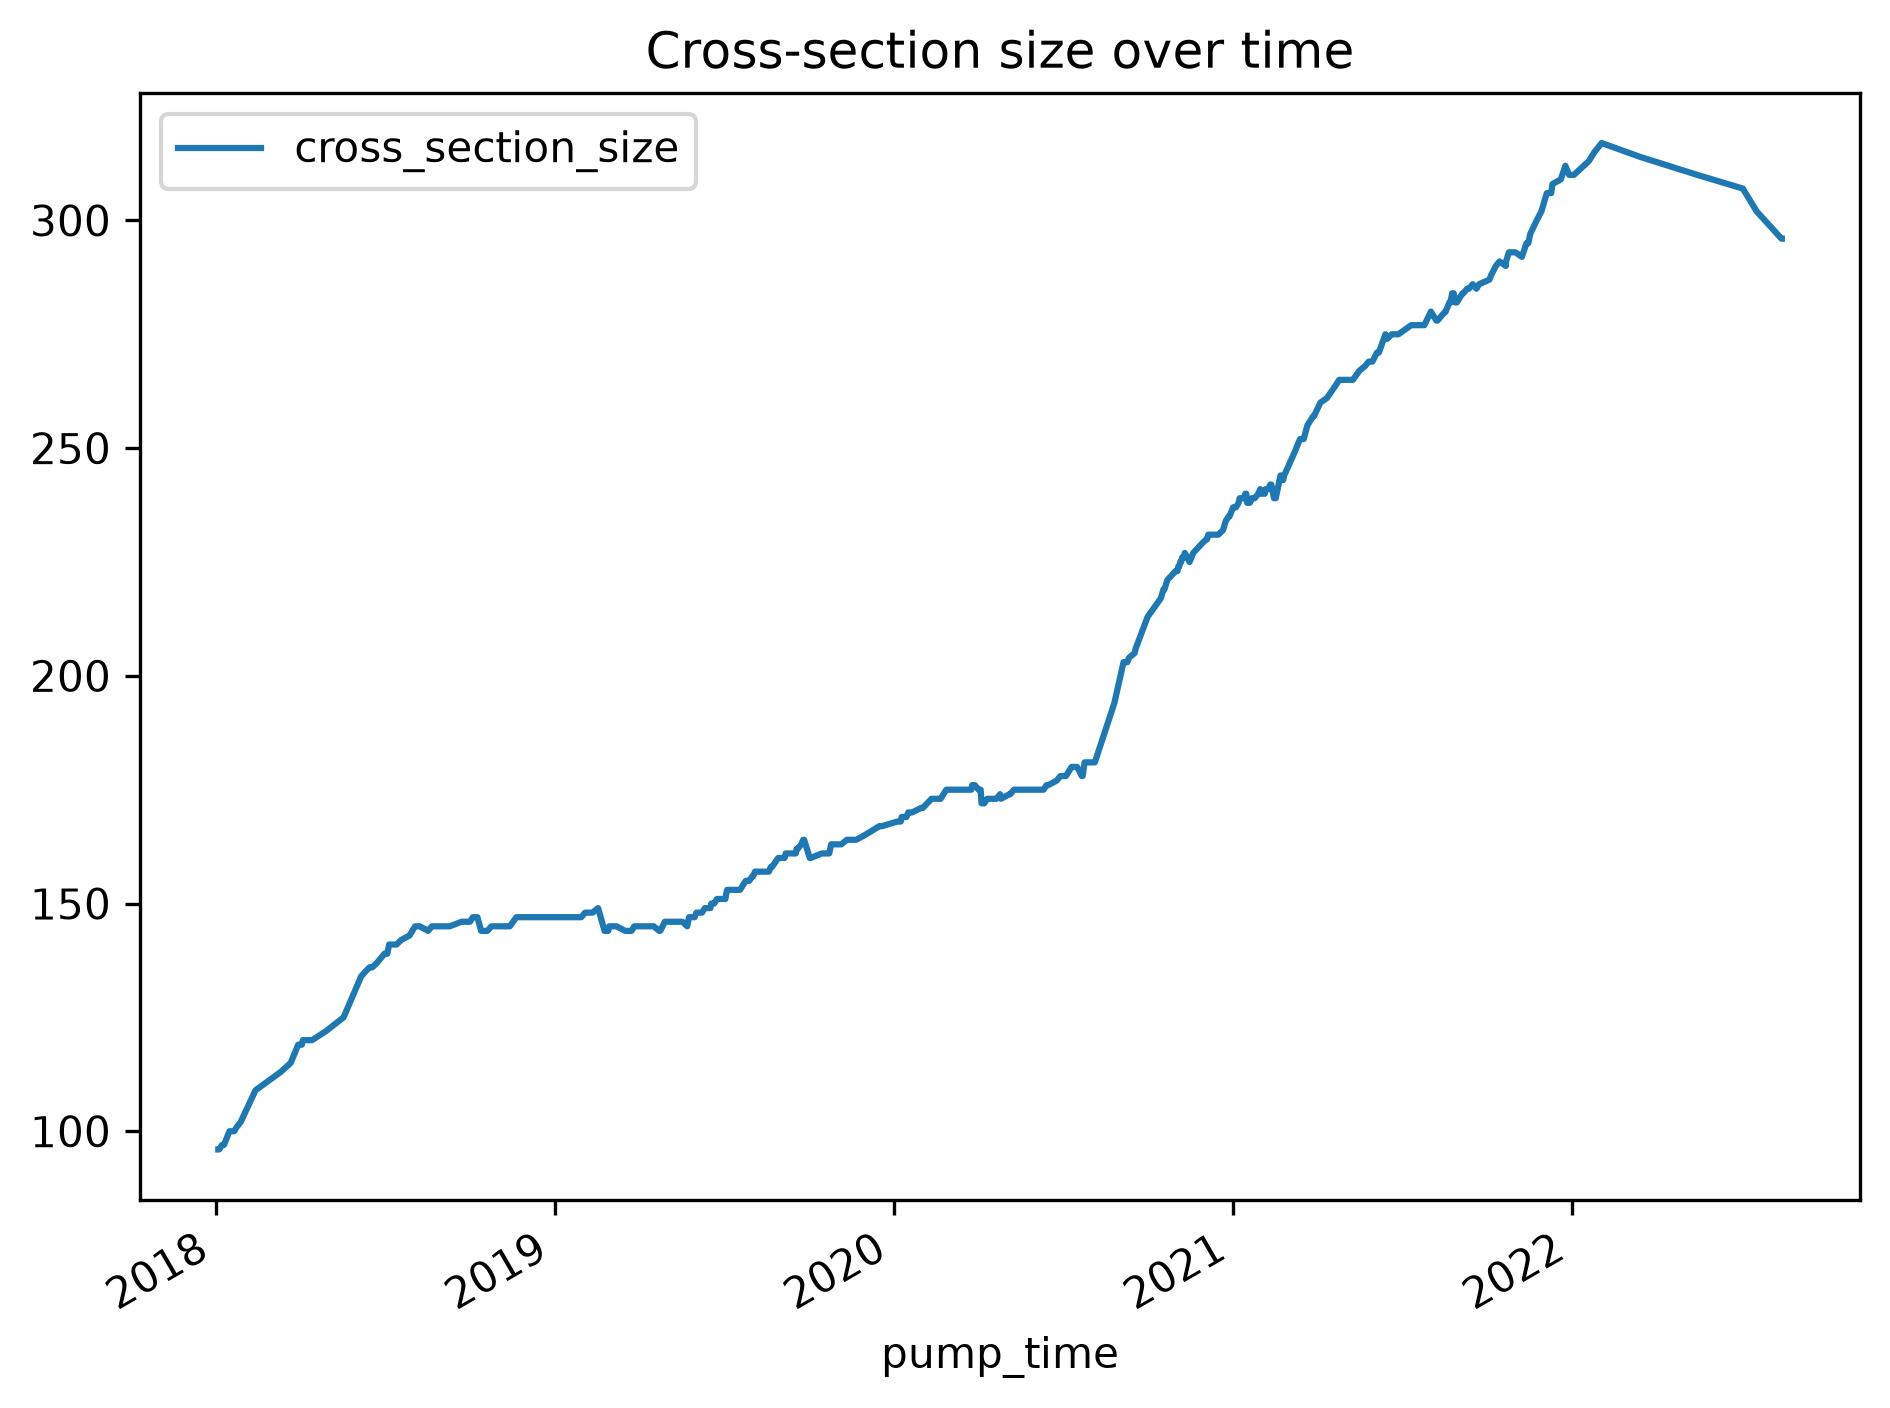
\includegraphics[scale=0.5]{images/cs_size.jpeg}
    \caption{Number of eligible Binance BTC-quoted pairs in the event cross-sections over time.}
    \label{fig:cross-section_size_over_time}
\end{figure}

We split the data into training, validation and testing samples by 2020-09-01 and 2021-05-01 respectively. Table~\ref{table:train_val_test_stats} describes the resulting datasets after the split: 

\begin{table}[!t]
    \centering
    \small
    \setlength{\tabcolsep}{5pt}
    \renewcommand{\arraystretch}{1.15}
    \caption{P\&D training, validation and test sample statistics.}
    \begin{tabular}{lrrr}
        \toprule
         & Train & Validation & Test \\
        \midrule
        Positive & 290 & 103 & 80 \\
        Negative & 44578 & 24274 & 22935 \\
        Total & 44868 & 24377 & 23015 \\
        Avg. Cross-section Size & 154.72 & 236.67 & 287.69 \\
        \bottomrule
    \end{tabular}
    \label{table:train_val_test_stats}
\end{table}

\subsection{Market data}

To enable comparison with existing research, we selected Binance as the sole exchange platform. We use Binance's public historical trade archive for every BTC-quoted pair needed by the 2018--2022 event manifest and its 30-day feature lookbacks.

A representative example of our collected data is presented in Table~\ref{table:collected_tick_data}.

\begin{table*}[!t]
    \centering
    \begin{tabular}{lrrrrr}
        \toprule
         & price & qty & time & isBuyerMaker & quote \\
        \midrule
        0 & 0.000002 & 2437.00 & 2022-07-15 15:00:02.422000 & True & 0.004240 \\
        1 & 0.000002 & 275.00& 2022-07-15 15:00:02.434000 & False & 0.000479 \\
        2 & 0.000002 & 1125.00 & 2022-07-15 15:00:22.884000 & True & 0.001946 \\
        3 & 0.000002 & 941.00 & 2022-07-15 15:00:52.277000 & True & 0.001628 \\
        4 & 0.000002 & 184.00 & 2022-07-15 15:00:52.277000 & True & 0.000318 \\
        \bottomrule
    \end{tabular}
    \caption{Structure of collected data: \textit{price} shows the price that the order was filled at, \textit{qty} is the amount of base asset traded, \textit{isBuyerMaker} indicates if the buyer's order related to this transaction was already in the orderbook: if True, the trade is classified as a Sell event and if False the trade is characterized as a Buy event.}
    \label{table:collected_tick_data}
\end{table*}


\subsection{Feature engineering}

We collected trade-level data as compressed daily archives for the required Binance pairs and dates. Because trading activity varies substantially across tickers and over time, the raw event streams are irregular and cannot be used directly as fixed-size inputs to standard machine-learning models. We therefore implemented a feature-generation pipeline that (i) decompresses and loads the relevant archives, (ii) partitions data into time-aligned windows, (iii) computes microstructure features summarizing pre-announcement order flow, and (iv) aggregates ticker-level features into an event-level cross-section associated with each pump. The pipeline is:

\begin{enumerate}
    \item Download trade-level data from Binance's public daily archive.
    \item For each pump event, construct the cross-section from tickers with at least one trade in the exact interval $[T-15\text{min}-1\text{d},T-15\text{min})$. Partition membership alone is insufficient because a daily partition can contain trades later than the decision time.
    \item For each eligible ticker, load 30 days of history ending at the decision cutoff and compute features over predefined half-open lookback windows $[T-15\text{min}-x,T-15\text{min})$. Hourly normalizer bars are re-anchored to the cutoff so every included bar is strictly pre-decision.
    \item Combine features for all tickers into a single event-level dataset and assign labels by adding \textit{is\_pumped}, which equals 1 for the pumped ticker and 0 otherwise.
\end{enumerate}

This modular pipeline supports feature construction with explicit decision-time boundaries. The implementation and instructions are available in \cite{code_github}. We group features into several categories, described below.

\subsubsection{Imbalance features}

Volume imbalance measures which side is more prevalent in trade data. It is the ratio of signed notional in the quote asset (negative for seller-initiated trades and positive for buyer-initiated trades) to total absolute quote notional. Values near $1$ indicate predominantly buyer-initiated flow and values near $-1$ predominantly seller-initiated flow.

\begin{equation}
    \text{Volume Imbalance} = \frac{\sum_{t \in \mathcal{T}}s_t p_t q_t}{\sum_{t \in \mathcal{T}}p_t q_t},
    \label{eq:volume_imbalance}
\end{equation}
where $p_tq_t$ is quote notional and $s_t\in\{-1,1\}$ is the taker-side sign at time $t$.

\subsubsection{Quote slippages}

We also created features based on slippage. Since we do not have information about order types, we cannot determine whether a trade was executed via a market or limit order; therefore, we treat slippage as a useful proxy for measuring market participants’ impatience. We follow the methodology used in prior work by grouping ticks by execution time. Given that we deal with highly illiquid markets—where the time between trades can be as long as 15 minutes—we can reasonably assume that aggregated ticks correspond to a single order. This allows us to estimate the price impact of the aggregated order. The intuition is as follows: if a market participant is willing to incur large slippage losses by submitting a large buy order, they likely want to build their position quickly, potentially in anticipation of the pump. Based on this idea, we compute slippage for each aggregated trade using the formula in \eqref{eq:slippage_loss} below:

\begin{equation}
    \begin{aligned}
        L &= \left|\sum_{i=1}^{N} q_i P_i-P_0\sum_{i=1}^{N}q_i\right|, \\
        L_{\mathrm{signed}} &= L\,\operatorname{sign}\!\left(\sum_{i=1}^{N}s_iq_i\right).
    \end{aligned}
    \label{eq:slippage_loss}
\end{equation}

where $q_i$, $P_i$, and $s_i$ are respectively the unsigned base quantity, execution price, and taker-side sign of the $i^{th}$ print in an aggregated timestamp group, and $P_0$ is its first execution price. Thus $L$ is the absolute difference between observed quote notional and the notional implied by filling the whole group at its first price; the sign is attached from net buyer- or seller-initiated base quantity. The slippage-imbalance feature is $\sum L_{\mathrm{signed}}/\sum L$. As an order consumes liquidity it can appear as a sequence of prints at worsening prices, so this statistic is intended to proxy how aggressively the group walks available liquidity.

\subsubsection{Arithmetic return features}

For each horizon $x$, the implementation computes the arithmetic return $10^4(p_{\mathrm{last}}/p_{\mathrm{prev}}-1)$ over $[T-15\text{min}-x,T-15\text{min})$. Return z-scores compare that window with the mean and sample standard deviation of decision-anchored hourly returns over the preceding 30 days. For $x\in\{5,15\}$ minutes, the exact-window return is converted to an hourly rate before standardization; for horizons of at least one hour, complete cutoff-anchored hourly bars are averaged. Thus the 5-minute, 15-minute, and 1-hour columns are distinct, while every numerator and normalizer remains strictly pre-decision.

\subsubsection{Power law features. Quantile spread of order sizes}

To summarize the tail of aggregated trade notionals $x\geq x_{\min}$ within each lookback window, we use the Pareto density

\begin{equation}
    f(x;\alpha,x_{\min})=(\alpha-1)x_{\min}^{\alpha-1}x^{-\alpha}, \qquad \alpha>1,
    \label{eq:powerlaw_pdf}
\end{equation}

where $x_{\min}$ is the minimum positive aggregated notional observed in the window. The code uses the closed-form maximum-likelihood estimate

\begin{equation}
    \hat{\alpha}=1+\frac{n}{\sum_{i=1}^{n}\log(x_i/x_{\min})}.
    \label{eq:powerlaw_ols}
\end{equation}

Smaller $\hat{\alpha}$ indicates a heavier notional tail. Before cross-sectional standardization, the implementation clips $\hat{\alpha}$ to the closed interval $[1,2]$. This deterministic bound handles degenerate short windows in which the denominator is zero (and the raw estimate is infinite) and limits the influence of extremely sparse tails. This is a fixed model-preprocessing rule, not a sample-dependent 95\% winsorization; no histogram-density regression or log--log OLS is performed.
\\ \\
All of the features discussed are further explained below (see Table~\ref{table:feature_descriptions}):

\begin{table*}[!t]
    \centering
    \small
    \renewcommand{\arraystretch}{1.25}
    \setlength{\tabcolsep}{10pt}
    \begin{tabular}{p{3cm}p{7cm}l}
        \hline
        \textbf{Feature} & \textbf{Description} & \textbf{Notation} \\
        \hline
        Asset return & return of the asset calculated over the window of size (T-15min-x, T-15min) prior to the pump announcement& \textit{asset\_return}[x]@\textit{t} \\
        \hline
        Standardized return & exact-window hourly-rate return (5m, 15m) or mean cutoff-anchored hourly return ($x\geq1$h), minus the 30-day hourly mean and divided by its standard deviation & \textit{asset\_return\_zscore}[x]@\textit{t} \\
        \hline
        Standardized volume in BTC & exact-window hourly-rate volume (5m, 15m) or mean cutoff-anchored hourly volume ($x\geq1$h), standardized by 30-day hourly moments & \textit{quote\_abs\_zscore}[x]@\textit{h} \\
        \hline
        Share of long trades & share of long trades as the ratio of number of long trades and all trades of this time window (T-15min-x, T-15min) & \textit{share\_of\_long\_trades}[x]@\textit{h} \\
        \hline
        Number of trades & number of timestamp-aggregated trades within $[T-15\mathrm{min}-x,T-15\mathrm{min})$ & \textit{num\_trades}[x]@\textit{h} \\
        \hline
        Flow imbalance ratio & volume imbalance ratio computed over the window of size (T-15min-x, T-15min) & \textit{flow\_imbalance}[x]@\textit{h} \\
        \hline
        Quote slippage imbalance ratio & imbalance ratio of slippages in BTC calculated over the same time window & \textit{slippage\_imbalance}[x]@\textit{t} \\
        \hline
        Powerlaw alpha & estimated alpha from powerlaw probability density function using the window of size (T-15min-x, T-15min) prior to the pump & \textit{powerlaw\_alpha}[x]@\textit{h} \\
        \hline
        Number of previous pumps & lifetime number of manifest events for this token strictly before the current announcement & \textit{num\_prev\_pump} \\
        \hline
    \end{tabular}
    \caption{These are the features included in all models. These features are used to describe historical dynamics of price and trading volume in the run up to the pump. $x \in \{5m, 15m, 1h, 2h, 4h, 12h, 1d, 2d, 7d, 14d\}$}
    \label{table:feature_descriptions}
\end{table*}

\subsection{Cross-sectional approach}
\label{sec:cs_standardization}

Given that our event dataset spans early 2018 through August 2022, we account for temporal heterogeneity by applying cross-sectional standardization. This approach reduces market-regime level shifts and focuses the models on relative cross-asset dynamics.

We apply cross-sectional standardization to the unbounded return, return-z-score, quote-volume-z-score, and power-law features. For each selected feature, we subtract its mean within an event and divide by its within-event sample standard deviation:

\begin{equation}
    X_{\text{standardized}} = \frac{X - \bar{X}_{CS}}{\bar{\sigma}_{CS}}
    \label{eq:cs_standardization}
\end{equation}

If a selected feature is constant within an event, it contains no relative ranking information and is mapped to zero; all-missing event columns remain missing for native handling or train-only imputation. We do not apply this second-stage transform to bounded imbalance/share features or to count features (trade counts and lifetime prior-pump count), whose nonnegative levels retain their direct interpretation. Fig.~\ref{fig:data_with_crossnorm} demonstrates the transform on a sample of five cross-sections for three selected numerical features:

\begin{figure*}[!t]
    \centering
    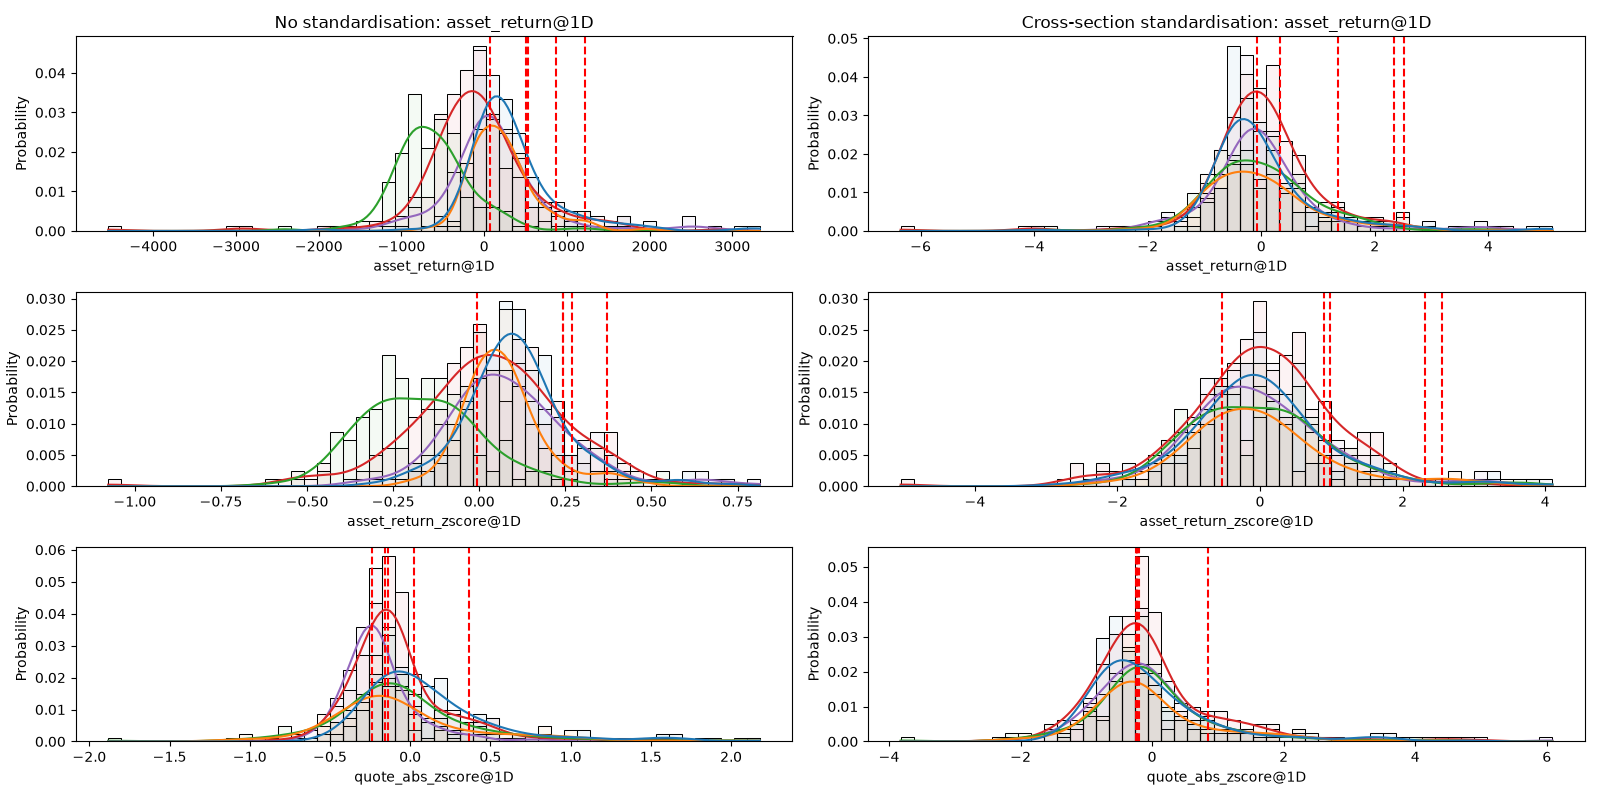
\includegraphics[scale=0.4]{images/cs_standardization_impact.png}
    \caption{Features with and without cross-sectional standardization: histograms and kernel-density estimates for five P\&D events. Applying standardization helps to align distributions more closely with one another across pumps.}
    \label{fig:data_with_crossnorm}
\end{figure*}

\section{Modelling}

In this section, we attempt to create a model able to label this fraudulent activity $15$ minutes before the announcement. As discussed earlier this is a challenging task due to high imbalance in the data. The task of finding manipulated assets can be designed as a binary classification problem where ``1'' implies that the asset is pumped and ``0'' that it is not. Therefore, we trained logistic regression, random forest, and CatBoost classifiers. The problem can also be formulated as learning to rank: the CatBoost ranker is supervised by each asset's realized arithmetic return over the first five minutes after announcement, ranked highest-first within its event cross-section (ordinal position 1 is the highest realized return). These post-announcement returns are labels only; the ranker's regressors are the same strictly pre-decision microstructure features used by the classifiers.

\subsection{Evaluation metrics}
\label{sec:evaluation_metrics}
Top@k is the probability that the ground-truth target occurs among a model's $k$ highest scores. In portfolio terms, it is the probability that a size-$k$ portfolio contains the pump target. Top@k\% replaces the fixed count with a percentage of each cross-section, controlling for the growth in Binance listings described in Section~\ref{section:pump_and_dump_data}. We use one notation convention throughout: Top@k and Top@k\% denote the fixed-count and percentage hit-rate curves; Top@kAUC and Top@k\%AUC denote their respective areas. A concrete threshold replaces $k$ in a point label, so Top@10 is the top-10 hit rate and Top@5\% is the top-5\% hit rate. The reported and optimized area in this study is Top@k\%AUC; Top@kAUC is reserved for an area over fixed-count $k$ and is not reported here.

The area under the Top@k\% curve (Top@k\%AUC) serves as our primary optimization target. In our setup we integrate the Top@k\% curve over the low-$k\%$ region $k\% \in (0,\,20\%]$ and normalize by the length of the integration range so the metric remains in $(0,1)$:
\begin{equation}
    \mathrm{Top@k\%AUC} \;=\; \frac{1}{0.20}\int_{0}^{0.20} \mathrm{Top@k\%}\,d(k\%).
    \label{eq:topkpauc}
\end{equation}
Restricting integration to the $(0,20\%]$ region is motivated by two considerations. First, it is the economically relevant region for a concentrated P\&D portfolio: a practical strategy holds at most the top $10$--$20\%$ of the cross-section in any given event. Second, all reasonably-trained models saturate above $k\% \approx 30\%$ and their Top@k\% curves converge, so integrating over the full $(0,1)$ range dilutes the metric with a large $k$ region where every model is close to $1$ and no longer discriminates between them. Truncating at $20\%$ makes Top@k\%AUC materially more sensitive to differences between models and to hyperparameter choices, which is the property we want from both an Optuna tuning target and an early-stopping signal inside CatBoost. Numerically, Top@k\%AUC values reported in this paper are therefore not directly comparable to AUCs integrated over $(0,1)$; a model that saturates quickly below $20\%$ can attain a Top@k\%AUC close to $0.8$ under this convention.

\subsubsection{Limitations of Top@k-based metrics}
While Top@k metrics are directly relevant for portfolio construction (how many assets must we hold to catch the pump?), they have limitations. They do not measure overall classification quality across the full score distribution and can mask poor calibration. A model may achieve high Top@k by ranking the pump target above most non-targets without producing well-separated probabilities. To address this, we complement Top@k with standard classification metrics.

\subsubsection{Standard classification metrics}
We additionally report three standard metrics on both the validation and test sets:
\begin{itemize}
    \item \textbf{PR-AUC:} Area under the precision--recall curve, which is more informative than receiver operating characteristic (ROC) AUC under extreme class imbalance~\cite{elkan2001cost}.
    \item \textbf{F1-score:} Harmonic mean of precision and recall, computed using a ``Top@1 per cross-section'' decision rule (predicting the highest-scored asset as positive).
    \item \textbf{Balanced accuracy:} Average of sensitivity and specificity, providing a class-imbalance-aware accuracy measure.
\end{itemize}

\subsection{Baseline model}

We use logistic regression as a simple baseline and compare it with a random-ranking model that selects candidate targets uniformly within each event cross-section. Class weights account for the imbalance between pump targets and other assets. Models are fitted on the training set and selected using validation Top@k\%AUC. Our primary metrics are Top@k and Top@k\%AUC, discussed in Section~\ref{section:results}.

\subsection{Training}
We used the training set to train the models. To reduce overfitting, tree depth was limited through the \textit{max\_depth} hyperparameter for both random forest and CatBoost models. We also applied early stopping for both CatBoost classifier and CatBoost ranker and used validation set to compute evaluation metrics. We created a custom evaluation metric Top@k\%AUC, this metric was used by the trainer to find the optimal number of boosted trees. We also set the number of early stopping rounds to 50 which implies that there is no improvement in Top@k\%AUC for more than 50 rounds, the training process will stop and the model will rollback to the best state. This was used in the training process of the model CatBoost classifier + Top@k\%AUC early stopping (early stopping model with custom evaluation metric).

The released notebook fixes the random seed to 42 for Optuna's TPE sampler, stochastic model training, SMOTE, and resampling. Tuning trials run sequentially, and CPU fitting uses one thread per model by default. L2 grid-search ties favor smaller $C$; the unpenalized logistic diagnostic uses deterministic Newton optimization. Run records include these settings, model parameters, feature order, input hashes, and software versions. Reproduction requires the same inputs and environment, with a fresh study when repeating hyperparameter tuning.

% BEGIN MODEL CONFIGURATION
We compare tuned L1 and L2 logistic regression, random forest, CatBoost, CatBoost with SMOTE, CatBoost ranker, and CatBoost + ES. L2 uses the L1 predictors and class weights and selects $C$ on validation Top@k\%AUC from 25 logarithmically spaced values between $10^{-6}$ and $10^2$, breaking ties toward smaller $C$. The selected value is $C=4.642\times10^{-5}$. The standalone unweighted, unpenalized statsmodels diagnostic is excluded from predictive comparisons.
% END MODEL CONFIGURATION

We validated the results using event-level resampling (Section~\ref{sec:significance}).

We also used SMOTE proposed by \cite{chawla2002smote} to tackle the problem of class imbalance. It allows to create new observations for the minority class to balance the dataset. Instead of copying existing minority points, it generates new, slightly different ones by interpolating between neighbors.


\section{Model Comparison}
\label{section:results}

\subsection{Validation Performance and Model Selection}
Table~\ref{table:validation_model_selection} compares seven tuned candidates using the same chronological split. CatBoost has the largest validation Top@k\%AUC ($0.653$). Validation guides model selection and early stopping; it is not an independent performance estimate. The selected model supplies all portfolio and price-impact results.

\begin{table*}[!t]
    \centering
    \small
    \setlength{\tabcolsep}{5pt}
    \renewcommand{\arraystretch}{1.15}
    \caption{Validation metrics for the seven tuned candidates. Top@k\%AUC selects the portfolio model; maxima are bold. F1 and balanced accuracy use one predicted target per event.}
    \resizebox{\ifdim\width>\textwidth\textwidth\else\width\fi}{!}{%
    \begin{tabular}{lrrrrrrrrrr}
        \toprule
        Model & Top@k\%AUC & Top@1 & Top@5 & Top@10 & Top@1\% & Top@5\% & Top@10\% & PR-AUC & F1 & Balanced accuracy \\
        \midrule
        CatBoost & \bfseries 0.653 & \bfseries 0.165 & \bfseries 0.417 & 0.524 & \bfseries 0.330 & 0.573 & 0.689 & \bfseries 0.089 & \bfseries 0.165 & \bfseries 0.581 \\
        CatBoost + ES & 0.646 & 0.126 & \bfseries 0.417 & \bfseries 0.553 & 0.252 & \bfseries 0.612 & 0.699 & 0.081 & 0.126 & 0.561 \\
        Logistic regression L2 & 0.611 & 0.097 & 0.311 & 0.456 & 0.243 & 0.505 & 0.670 & 0.057 & 0.097 & 0.547 \\
        Logistic regression L1 & 0.610 & 0.107 & 0.282 & 0.456 & 0.214 & 0.505 & \bfseries 0.709 & 0.057 & 0.107 & 0.552 \\
        Random forest & 0.565 & 0.117 & 0.320 & 0.417 & 0.262 & 0.456 & 0.602 & 0.084 & 0.117 & 0.556 \\
        CatBoost + SMOTE & 0.524 & 0.097 & 0.233 & 0.379 & 0.214 & 0.408 & 0.583 & 0.075 & 0.097 & 0.547 \\
        CatBoost ranker & 0.501 & 0.078 & 0.330 & 0.398 & 0.204 & 0.427 & 0.534 & 0.038 & 0.078 & 0.537 \\
        \bottomrule
    \end{tabular}
    }
    \label{table:validation_model_selection}
\end{table*}


\begin{figure*}[!t]
    \centering
    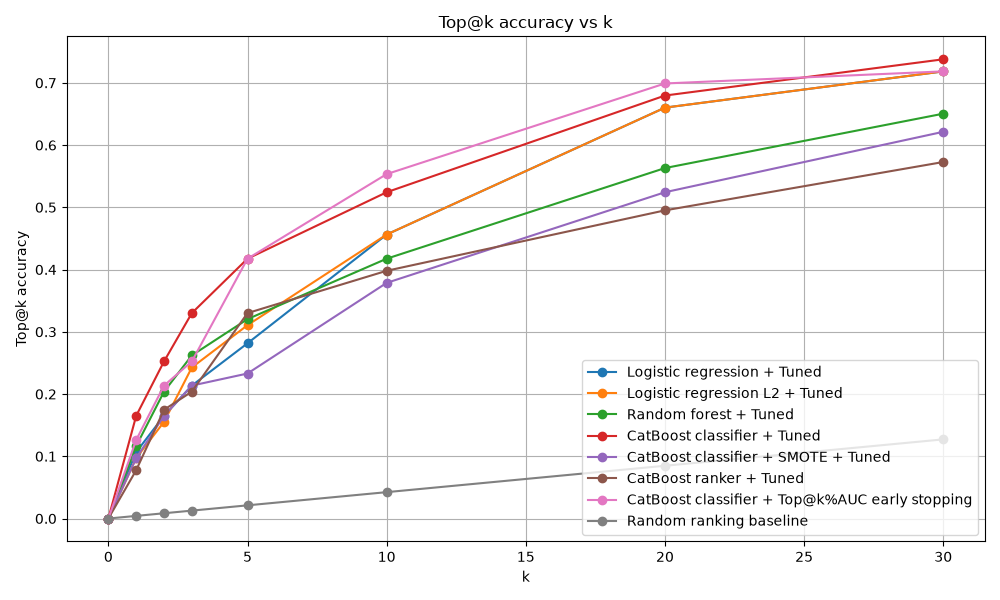
\includegraphics[width=\textwidth]{images/topk_accuracy_validation.png}
    \caption{Validation Top@k accuracy for the seven tuned candidates and the random-ranking baseline.}
    \label{fig:validation_topk}
\end{figure*}

\begin{figure*}[!t]
    \centering
    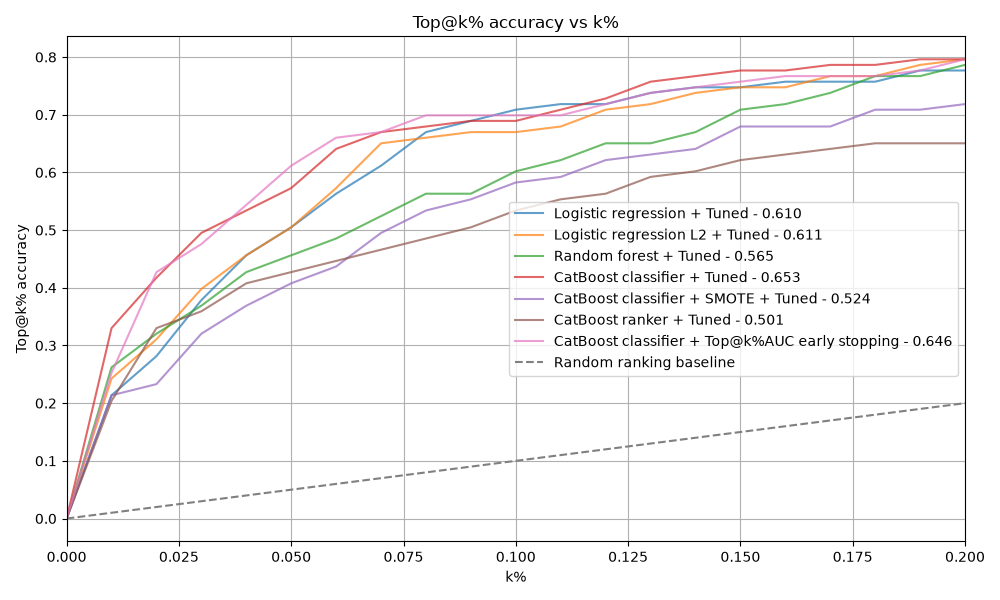
\includegraphics[width=\textwidth]{images/topkp_auc_validation.png}
    \caption{Validation Top@k\% curves and normalized Top@k\%AUC. Model selection uses this validation criterion.}
    \label{fig:validation_topkp}
\end{figure*}

\begin{figure*}[!t]
    \centering
    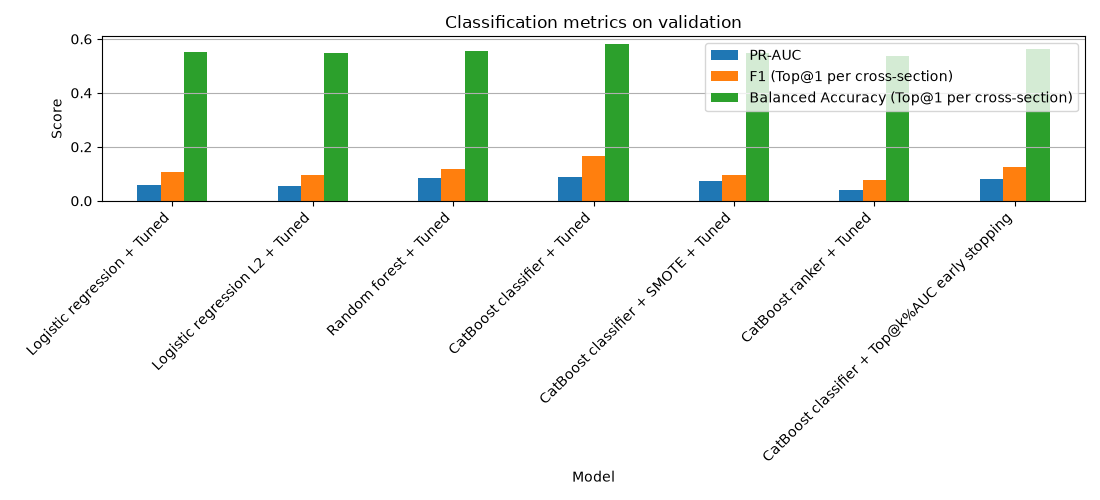
\includegraphics[width=\textwidth]{images/classification_metrics_validation.png}
    \caption{Validation PR-AUC, F1 and balanced accuracy for the seven candidates; classification uses one predicted target per event.}
    \label{fig:validation_classification}
\end{figure*}

\subsection{Test Ranking Performance}
Tables~\ref{table:results_topk} and~\ref{table:results_topkp} report target inclusion at fixed portfolio sizes and cross-section fractions. CatBoost achieves Top@1 $0.188$, Top@5 $0.450$ (36 of 80 events), and Top@10 $0.500$. Test comparisons describe the selected models; they do not change the validation selection rule.

\begin{table*}[!t]
    \centering
    \small
    \setlength{\tabcolsep}{5pt}
    \renewcommand{\arraystretch}{1.15}
    \caption{Test Top@k accuracy for the seven tuned candidates.}
    \resizebox{\ifdim\width>\textwidth\textwidth\else\width\fi}{!}{%
    \begin{tabular}{lrrrrrr}
        \toprule
        Model & Top@1 & Top@2 & Top@5 & Top@10 & Top@20 & Top@30 \\
        \midrule
        CatBoost & 0.188 & 0.275 & 0.450 & 0.500 & 0.662 & 0.713 \\
        CatBoost + ES & 0.125 & 0.212 & 0.438 & 0.575 & 0.688 & 0.750 \\
        Logistic regression L2 & 0.113 & 0.200 & 0.400 & 0.588 & 0.713 & 0.787 \\
        Logistic regression L1 & 0.100 & 0.150 & 0.438 & 0.550 & 0.713 & 0.750 \\
        Random forest & 0.087 & 0.163 & 0.312 & 0.450 & 0.575 & 0.675 \\
        CatBoost + SMOTE & 0.050 & 0.163 & 0.250 & 0.325 & 0.438 & 0.537 \\
        CatBoost ranker & 0.050 & 0.125 & 0.212 & 0.400 & 0.537 & 0.588 \\
        \bottomrule
    \end{tabular}
    }
    \label{table:results_topk}
\end{table*}

\begin{table*}[!t]
    \centering
    \small
    \setlength{\tabcolsep}{5pt}
    \renewcommand{\arraystretch}{1.15}
    \caption{Test Top@k\% accuracy for the seven tuned candidates.}
    \resizebox{\ifdim\width>\textwidth\textwidth\else\width\fi}{!}{%
    \begin{tabular}{lrrrrrr}
        \toprule
        Model & Top@1\% & Top@2\% & Top@5\% & Top@10\% & Top@20\% & Top@50\% \\
        \midrule
        CatBoost & 0.388 & 0.450 & 0.625 & 0.713 & 0.875 & 0.963 \\
        CatBoost + ES & 0.312 & 0.500 & 0.662 & 0.750 & 0.863 & 0.963 \\
        Logistic regression L2 & 0.312 & 0.500 & 0.637 & 0.787 & 0.875 & 0.950 \\
        Logistic regression L1 & 0.287 & 0.500 & 0.625 & 0.725 & 0.887 & 0.963 \\
        Random forest & 0.263 & 0.375 & 0.512 & 0.662 & 0.775 & 0.950 \\
        CatBoost + SMOTE & 0.200 & 0.275 & 0.412 & 0.537 & 0.750 & 0.900 \\
        CatBoost ranker & 0.163 & 0.263 & 0.500 & 0.588 & 0.688 & 0.912 \\
        \bottomrule
    \end{tabular}
    }
    \label{table:results_topkp}
\end{table*}

The random-ranking baseline averages $\min(k,T_i)/T_i$ across events, where $T_i$ is the number of eligible assets in event $i$. Normalized Top@k\%AUC integrates the inclusion curve from 0 to 20\% in 0.5\% increments, as in Eq.~\ref{eq:topkpauc}.

\begin{figure*}[!t]
    \centering
    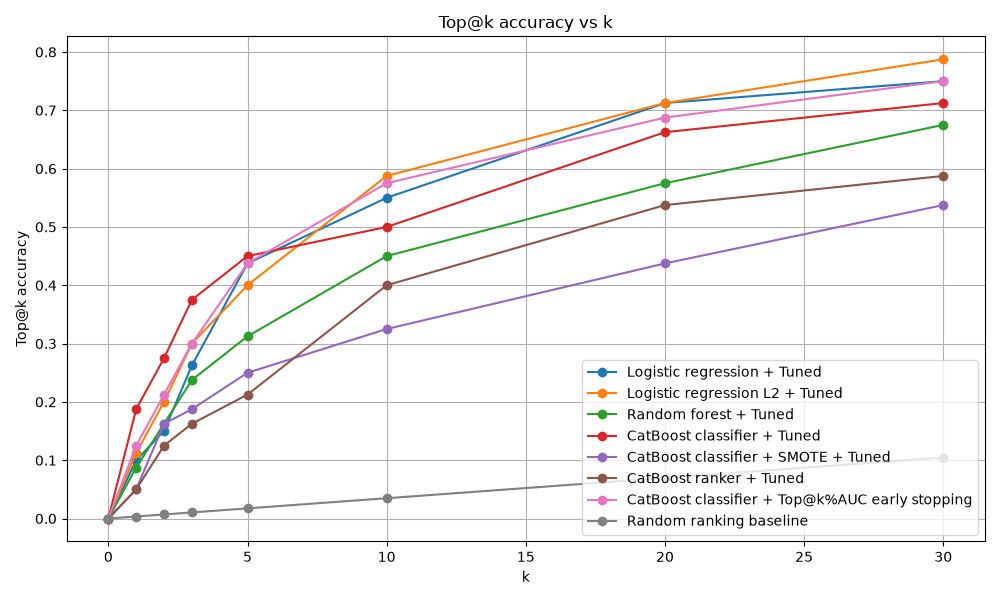
\includegraphics[width=\textwidth]{images/topk_accuracy_test.png}
    \caption{Test Top@k accuracy and the event-specific random-ranking baseline.}
    \label{fig:results_topk}
\end{figure*}

\begin{figure*}[!t]
    \centering
    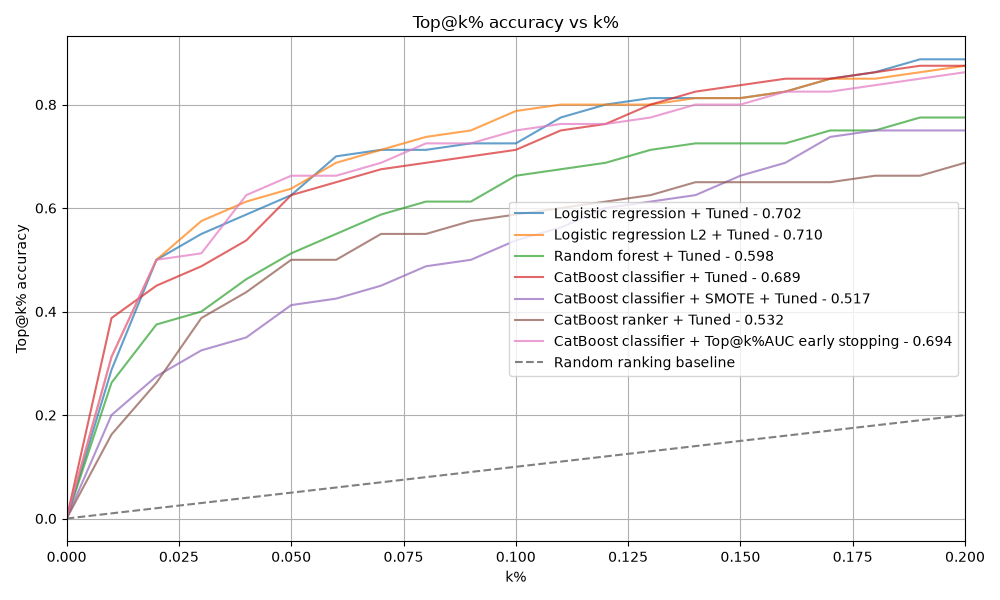
\includegraphics[width=\textwidth]{images/topkp_auc_test.png}
    \caption{Test Top@k\% accuracy curves and normalized Top@k\%AUC for the same seven fitted candidates.}
    \label{fig:results_topkp}
\end{figure*}

L2 logistic regression has the largest test Top@k\%AUC point estimate ($0.710$), followed by L1 logistic regression ($0.702$), CatBoost + ES ($0.694$), CatBoost ($0.689$), and random forest ($0.598$). Statistical comparisons use paired event resampling in Section~\ref{sec:significance}.

\subsection{Classification Metrics}
Fig.~\ref{fig:classification_metrics} reports PR-AUC, F1 and balanced accuracy. F1 and balanced accuracy use the Top@1-per-event rule, so these scores measure the identification of one target within each event rather than an arbitrary probability threshold.

CatBoost has the highest test PR-AUC ($0.0799$). CatBoost has PR-AUC $0.0799$, F1 $0.1875$ and balanced accuracy $0.5923$.

\begin{figure*}[!t]
    \centering
    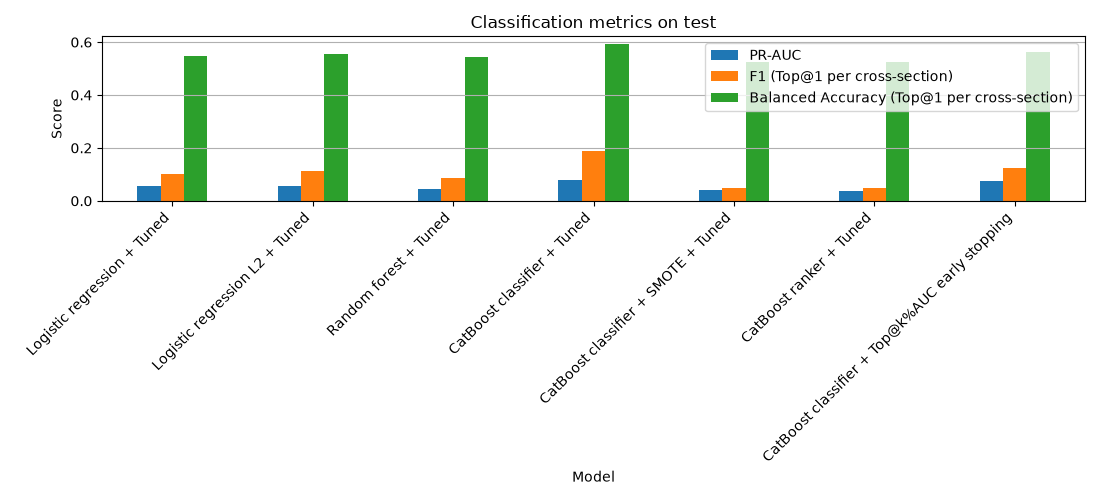
\includegraphics[width=\textwidth]{images/classification_metrics_test.png}
    \caption{Test classification metrics for the seven tuned candidates.}
    \label{fig:classification_metrics}
\end{figure*}

\subsection{SMOTE and Ranking Models}
CatBoost with SMOTE attains test Top@1 $5.00\%$ and Top@k\%AUC $0.517$, below the leading class-weighted classifiers. With 81 predictors and 290 positive training events, synthetic interpolation may mix observations with different event-specific reference distributions. This is a plausible explanation, rather than a causal test, and is consistent with known limitations of SMOTE in high-dimensional data~\cite{blagus2013smote}.

The CatBoost ranker attains test Top@1 $5.00\%$ and Top@k\%AUC $0.532$. It learns an ordering of post-announcement returns, whereas evaluation asks whether the single manipulation target appears near the top. Noise in the returns of other assets and the mismatch between these objectives may explain its weaker performance. Ranking advantages in other financial applications~\cite{poh_ltr} do not automatically transfer to this sample.

\subsection{Interpretation of CatBoost + ES}
Fig.~\ref{fig:catboost_fi} reports CatBoost PredictionValuesChange for CatBoost + ES fitted on all training events. Table~\ref{table:feature_importance_quantiles} summarizes the 15 largest median importances across the 25 training-subset fits in Section~\ref{sec:robustness}. These describe the fitted prediction function; they are not causal effects or evidence of manipulation by themselves.

\begin{figure*}[!t]
    \centering
    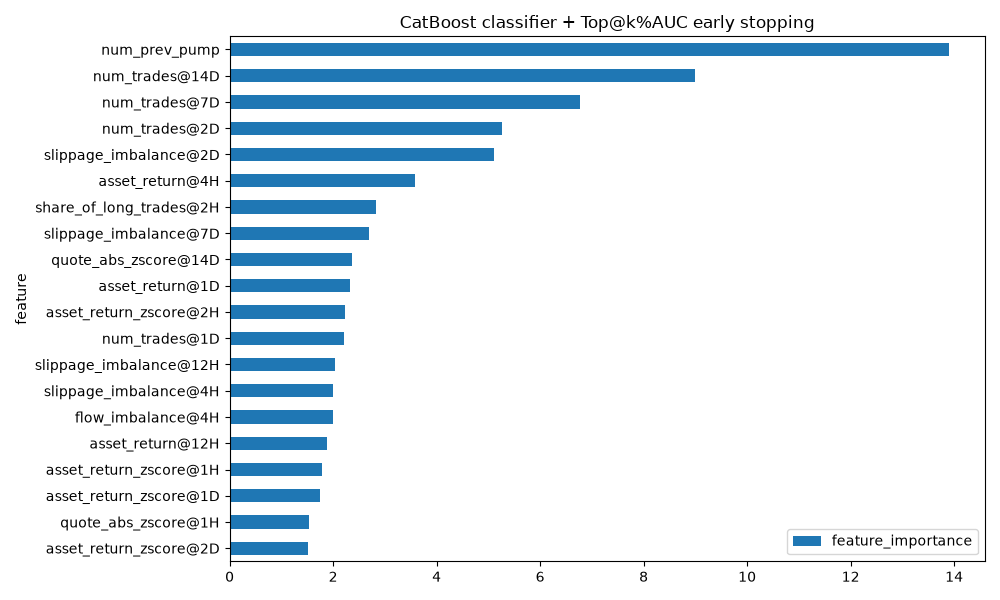
\includegraphics[width=\textwidth]{images/feature_importances.png}
    \caption{Feature importance for the CatBoost + ES model fitted on all training events.}
    \label{fig:catboost_fi}
\end{figure*}

\begin{table*}[!t]
    \centering
    \small
    \setlength{\tabcolsep}{5pt}
    \renewcommand{\arraystretch}{1.15}
    \caption{CatBoost PredictionValuesChange quantiles across 25 fits on random 70\% training-event subsets. Rows are ordered by median importance.}
    \resizebox{\ifdim\width>\textwidth\textwidth\else\width\fi}{!}{%
    \begin{tabular}{lrrrrr}
        \toprule
        Feature & 10\% & 25\% & Median & 75\% & 90\% \\
        \midrule
        num\_prev\_pump & 9.70 & 11.35 & 12.89 & 16.86 & 20.92 \\
        num\_trades@7D & 3.17 & 5.06 & 8.73 & 13.11 & 16.11 \\
        num\_trades@2D & 5.03 & 5.23 & 7.19 & 9.75 & 12.79 \\
        num\_trades@14D & 1.48 & 3.32 & 4.97 & 8.84 & 11.37 \\
        slippage\_imbalance@12H & 0.92 & 2.15 & 3.38 & 5.22 & 7.00 \\
        asset\_return@12H & 1.26 & 1.65 & 2.56 & 3.23 & 3.95 \\
        asset\_return@1D & 1.05 & 1.37 & 2.43 & 3.19 & 4.35 \\
        quote\_abs\_zscore@1H & 0.30 & 0.92 & 2.38 & 2.83 & 3.55 \\
        slippage\_imbalance@2D & 0.71 & 1.39 & 2.24 & 3.40 & 4.73 \\
        asset\_return@4H & 0.73 & 1.71 & 2.22 & 3.09 & 3.84 \\
        asset\_return\_zscore@2H & 0.57 & 1.31 & 2.14 & 3.10 & 4.52 \\
        slippage\_imbalance@4H & 0.00 & 0.36 & 1.69 & 1.95 & 2.49 \\
        asset\_return@2H & 0.08 & 0.69 & 1.54 & 2.25 & 2.34 \\
        asset\_return\_zscore@1H & 0.42 & 1.12 & 1.51 & 2.47 & 4.13 \\
        slippage\_imbalance@1D & 0.07 & 0.46 & 1.49 & 2.61 & 4.27 \\
        \bottomrule
    \end{tabular}
    }
    \label{table:feature_importance_quantiles}
\end{table*}

\subsection{Statistical Significance}
\label{sec:significance}
We validate the results using 10{,}000 paired bootstrap samples of the 80 whole test events. All candidate assets stay with their event, repeated events retain their multiplicity, and identical event draws are used for all seven fixed models. Models are not retrained within this bootstrap. The percentile intervals quantify sampling uncertainty conditional on the fitted models and assume independent events; they do not account for training uncertainty, temporal dependence or prior test inspection.

Pairwise differences use a two-sided null distribution centered at zero, an add-one Monte Carlo correction and Holm adjustment across the 21 unordered model pairs. We use paired differences rather than marginal-interval overlap to assess significance.

\begin{table}[!t]
    \centering
    \small
    \setlength{\tabcolsep}{5pt}
    \renewcommand{\arraystretch}{1.15}
    \caption{Test sample Top@k\%AUC point estimates and 95\% percentile intervals from 10{,}000 paired event resamples.}
    \begin{tabular}{lrr}
        \toprule
        Model & Top@k\%AUC & 95\% CI \\
        \midrule
        Logistic regression L2 & 0.710 & $[0.633,\,0.784]$ \\
        Logistic regression L1 & 0.702 & $[0.625,\,0.776]$ \\
        CatBoost + ES & 0.694 & $[0.614,\,0.771]$ \\
        CatBoost & 0.689 & $[0.612,\,0.764]$ \\
        Random forest & 0.598 & $[0.513,\,0.682]$ \\
        CatBoost ranker & 0.532 & $[0.442,\,0.621]$ \\
        CatBoost + SMOTE & 0.517 & $[0.433,\,0.601]$ \\
        \bottomrule
    \end{tabular}
    \label{table:significance_ci}
\end{table}

CatBoost minus L1 logistic regression has AUC difference $-0.0133$, paired 95\% CI $[-0.0678,\,0.0380]$, two-sided $p=0.6137$ and Holm-adjusted $p=1.000$. Against L2 logistic regression, the difference is $-0.0212$, paired 95\% CI $[-0.0794,\,0.0345]$, two-sided $p=0.4570$ and Holm-adjusted $p=1.000$. Against CatBoost + ES, the difference is $-0.0055$, paired 95\% CI $[-0.0362,\,0.0259]$, two-sided $p=0.7363$ and Holm-adjusted $p=1.000$. The L1-minus-L2 difference is $-0.0080$, paired 95\% CI $[-0.0264,\,0.0112]$, two-sided $p=0.4100$ and Holm-adjusted $p=1.000$. These comparisons do not establish superiority or equivalence. Model selection remains based on validation performance.

The selected model's differences against random forest, CatBoost with SMOTE and the ranker are, respectively: $0.0903$, paired 95\% CI $[0.0286,\,0.1542]$, two-sided $p=0.0045$ and Holm-adjusted $p=0.049$; $0.1713$, paired 95\% CI $[0.1094,\,0.2331]$, two-sided $p=0.0001$ and Holm-adjusted $p=0.002$; and $0.1564$, paired 95\% CI $[0.0747,\,0.2389]$, two-sided $p=0.0003$ and Holm-adjusted $p=0.004$. These three differences remain significant after Holm correction at the 5\% level, subject to the sampling assumptions and test-inspection limitation above.

\begin{figure*}[!t]
    \centering
    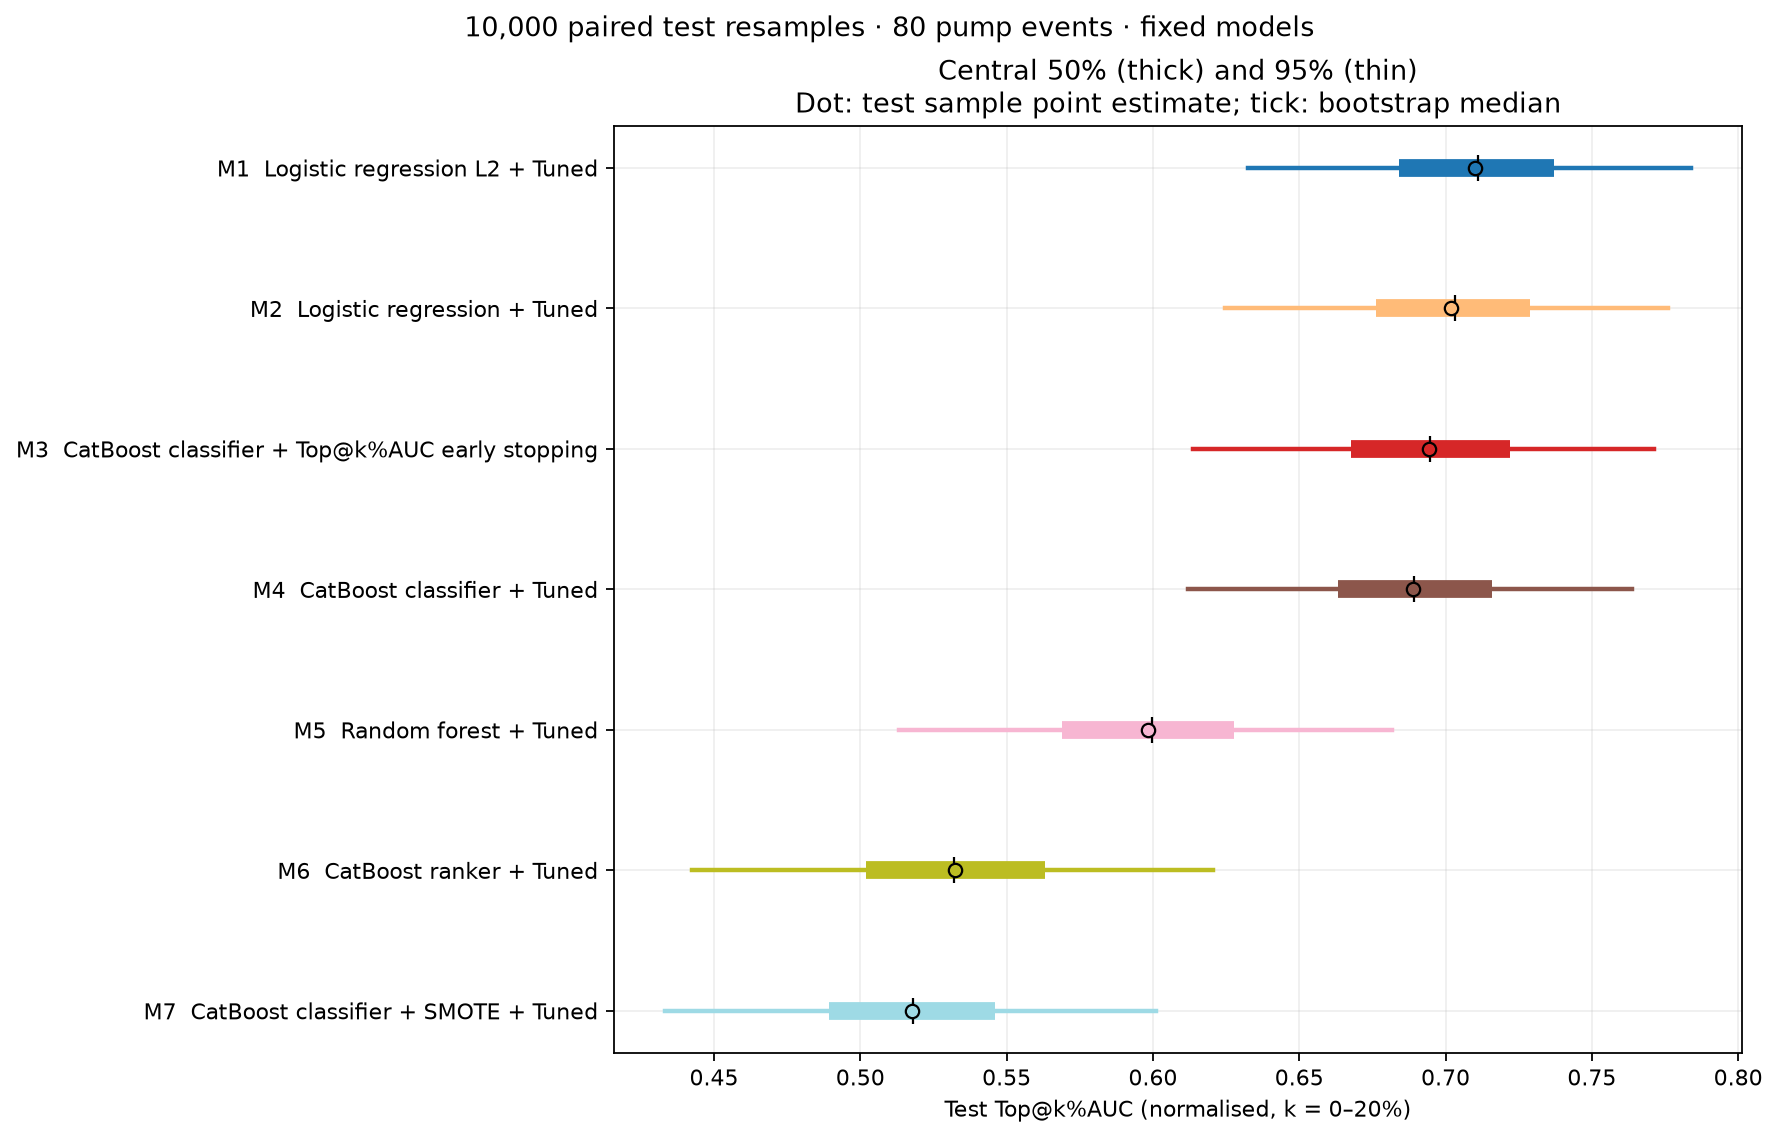
\includegraphics[width=\textwidth]{images/auc_distributions.png}
    \caption{Test Top@k\%AUC bootstrap distributions for the seven fixed models: central 50\% and 95\% intervals, medians and test sample point estimates. All models use the same 10{,}000 event draws.}
    \label{fig:auc_bootstrap}
\end{figure*}

\begin{figure*}[!t]
    \centering
    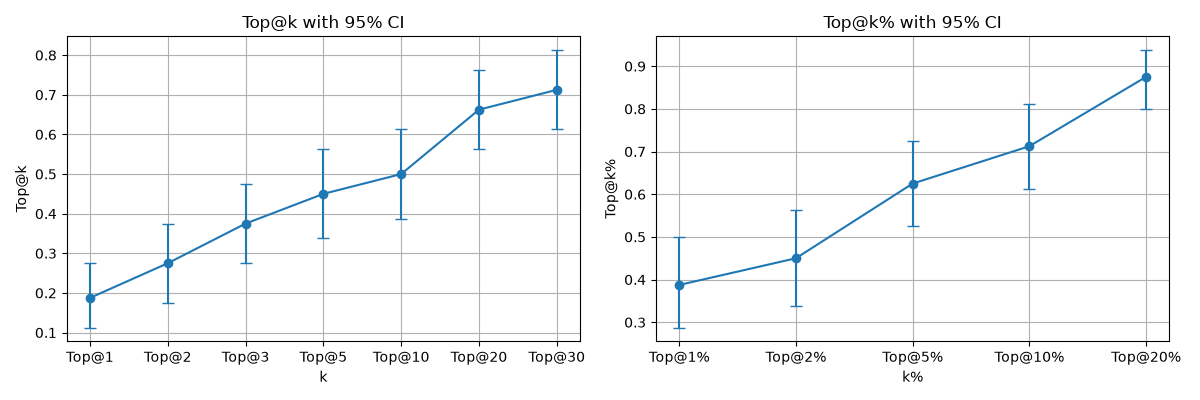
\includegraphics[width=\textwidth]{images/significance_bootstrap_ci.png}
    \caption{CatBoost test Top@k and Top@k\% point estimates with 95\% intervals from 10{,}000 whole-event resamples.}
    \label{fig:bootstrap_ci}
\end{figure*}

\subsection{Robustness Analysis}
\label{sec:robustness}
\subsubsection{Training-event sensitivity}
We retrain CatBoost + ES 25 times on random 70\% subsets of the training events, keeping hyperparameters and validation/test membership fixed. Table~\ref{table:robustness_summary} and Fig.~\ref{fig:robustness_distribution} summarize test performance. Mean AUC is $0.688$, its standard deviation is $0.014$, and the central 80\% range is $[0.668,\,0.702]$.

\begin{table}[!t]
    \centering
    \small
    \setlength{\tabcolsep}{5pt}
    \renewcommand{\arraystretch}{1.15}
    \caption{Test performance across 25 random 70\% training-event subset fits of CatBoost + ES.}
    \begin{tabular}{lrrr}
        \toprule
        Metric & Mean & Std & [10\%, 90\%] \\
        \midrule
        Top@k\%AUC & 0.688 & 0.014 & [0.668, 0.702] \\
        Top@1\% & 0.326 & 0.047 & [0.260, 0.375] \\
        Top@2\% & 0.469 & 0.038 & [0.427, 0.512] \\
        Top@5\% & 0.629 & 0.028 & [0.593, 0.650] \\
        Top@10\% & 0.747 & 0.021 & [0.725, 0.775] \\
        Top@20\% & 0.846 & 0.025 & [0.825, 0.863] \\
        \bottomrule
    \end{tabular}
    \label{table:robustness_summary}
\end{table}

\begin{figure*}[!t]
    \centering
    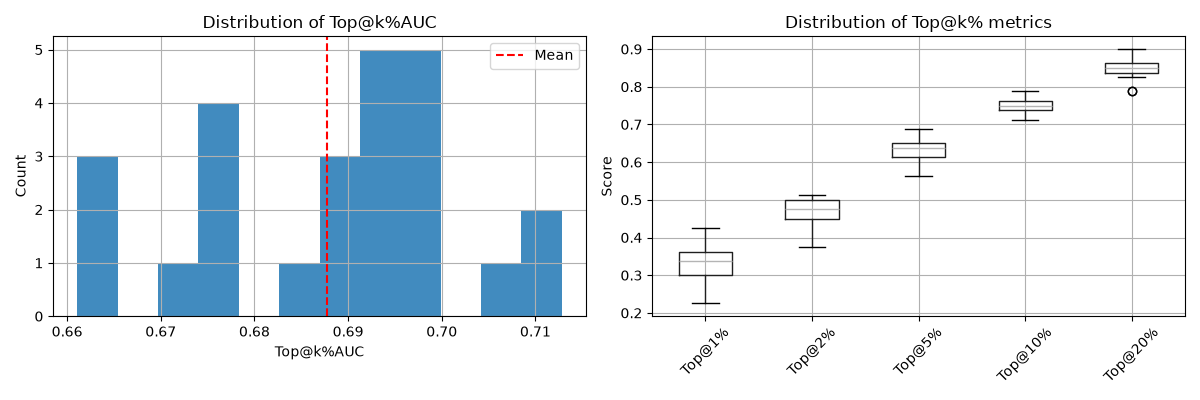
\includegraphics[width=\textwidth]{images/robustness_metrics_distribution.png}
    \caption{Distribution of test ranking metrics across 25 CatBoost + ES fits on different 70\% training-event subsets, with validation and test membership fixed.}
    \label{fig:robustness_distribution}
\end{figure*}

The corresponding L2 logistic regression analysis keeps the selected penalty, $C$, and class weights fixed. Its mean test AUC is $0.707$, standard deviation $0.007$, and central 80\% range $[0.698,\,0.715]$. Preprocessing is fitted using each training subset. These experiments measure conditional training sensitivity and do not provide independent external validation.

\subsubsection{Temporal subperiod analysis}
Using June~1, 2022 as the subperiod boundary, the early test period contains 76 events and has CatBoost AUC $0.695$. The late period contains only four events and is excluded by the minimum of ten events per subperiod. This sample therefore does not support a reliable claim about bear-market or cross-regime performance.

\section{Portfolio strategy}
\label{sec:portfolio}

This section evaluates a portfolio strategy inspired by \cite{pd_anatomy}, with modified construction and execution assumptions tailored to the proposed scoring framework. Authors of \cite{pd_anatomy} proposed using trained classification models to produce logits for each asset in the cross-section, then construct a portfolio of assets that have their logit of being pumped above some threshold. They also proposed using weights of the portfolio proportional to the logits produced by the model. They backtested their strategy using the following assumptions: assets that are not pumped do not change in price over the pump, authors buy at open price of the last hourly candle prior to the pump and are able to sell at half of pump's max return. They backtested their strategy using the test sample from October 29, 2018 to January 11, 2019 and were able to achieve a return of 60\% over approximately two months. We extend this approach by constructing portfolios from the proposed model scores and by adopting more conservative execution assumptions. 

We propose using models tuned for Top@k\%AUC which will ensure that the models are optimized not only for Top@1 accuracy but for any arbitrary values of k. We relaxed some assumptions of \cite{pd_anatomy} in the way we trade our portfolios, the timeline of how we trade each pump is described below:

\begin{enumerate}
  \item Rank tickers by model logits (descending).
  \item Select the Top@k set of tickers.
  \item Submit equal-weight entries 15 minutes before the announcement and fill each at its first subsequent pre-announcement trade; omit a leg if no such trade occurs. The omitted leg's fixed $1/k$ weight remains in cash and is not redistributed.
  \item Hold until the announcement; if not pumped, sell at the announcement; if pumped, sell 1 minute after the pump.
  \item Liquidate the complete acquired base-asset quantity, convert the BTC proceeds to USDT at the exit-time completed indicative rate, and subtract a $25$ bp ($0.25\%$) round-trip cost from entry capital.
\end{enumerate}


We use the validation-selected CatBoost model for every portfolio and price-impact analysis. We compare $k\in\{1,2,5,10,20,30\}$ and retain $k=5$ for order-size sensitivity. At $k=5$, target inclusion is $45.00\%$ (36 of 80 events), exactly matching Top@5 in Table~\ref{table:results_topk}.

For each size, we generate 10{,}000 random portfolios. At each event, $k$ different eligible assets are selected uniformly and assigned equal weights, using common random asset orders across sizes. Trading rules, USDT conversion and the 25 bp round-trip cost match the model strategy. Unfilled allocations remain in cash. Events stay in chronological order and returns are summed without reinvestment. Annualized statistics use zero-filled daily returns over the same calendar and 365 days per year; each statistic is computed for each draw before averaging.

At $k=5$, CatBoost cumulative return is $97.46\%$ and Sharpe is $2.86$. Random selection has mean return $-10.22\%$ with a central 95\% range of $[-23.29\%,\,20.90\%]$ and mean target inclusion $1.74\%$. These ranges describe random selection within the observed test period, not event-bootstrap confidence intervals or confirmatory significance tests.
\begin{table*}[!t]
    \centering
    \small
    \setlength{\tabcolsep}{5pt}
    \renewcommand{\arraystretch}{1.15}
    \caption{Portfolio performance without size-dependent impact. Random rows average statistics computed separately for 10{,}000 draws. All returns are decimal fractions.}
    \resizebox{\ifdim\width>\textwidth\textwidth\else\width\fi}{!}{%
    \begin{tabular}{lrrrrr}
        \toprule
        Portfolio & Avg. event return & Cumulative return & Annualized return & Annualized volatility & Sharpe \\
        \midrule
        CatBoost $k=1$ & 0.0091 & 0.7281 & 0.5642 & 0.6839 & 0.8250 \\
        CatBoost $k=2$ & 0.0141 & 1.1268 & 0.8732 & 0.4534 & 1.9258 \\
        CatBoost $k=5$ & 0.0122 & 0.9746 & 0.7553 & 0.2643 & 2.8581 \\
        CatBoost $k=10$ & 0.0058 & 0.4654 & 0.3607 & 0.2010 & 1.7943 \\
        CatBoost $k=20$ & 0.0043 & 0.3469 & 0.2688 & 0.1293 & 2.0796 \\
        CatBoost $k=30$ & 0.0025 & 0.1998 & 0.1548 & 0.0877 & 1.7648 \\
        Random $k=1$ & -0.0013 & -0.1023 & -0.0793 & 0.1313 & -1.2805 \\
        Random $k=2$ & -0.0013 & -0.1015 & -0.0787 & 0.1089 & -1.3999 \\
        Random $k=5$ & -0.0013 & -0.1022 & -0.0792 & 0.0843 & -1.4597 \\
        Random $k=10$ & -0.0013 & -0.1029 & -0.0798 & 0.0699 & -1.4881 \\
        Random $k=20$ & -0.0013 & -0.1033 & -0.0801 & 0.0587 & -1.5473 \\
        Random $k=30$ & -0.0013 & -0.1035 & -0.0802 & 0.0536 & -1.6031 \\
        BTCUSDT buy-and-hold & --- & -0.5727 & -0.4448 & 0.7340 & -0.6060 \\
        \bottomrule
    \end{tabular}
    }
    \label{table:performance_by_k}
\end{table*}
\begin{figure*}[!t]
    \centering
    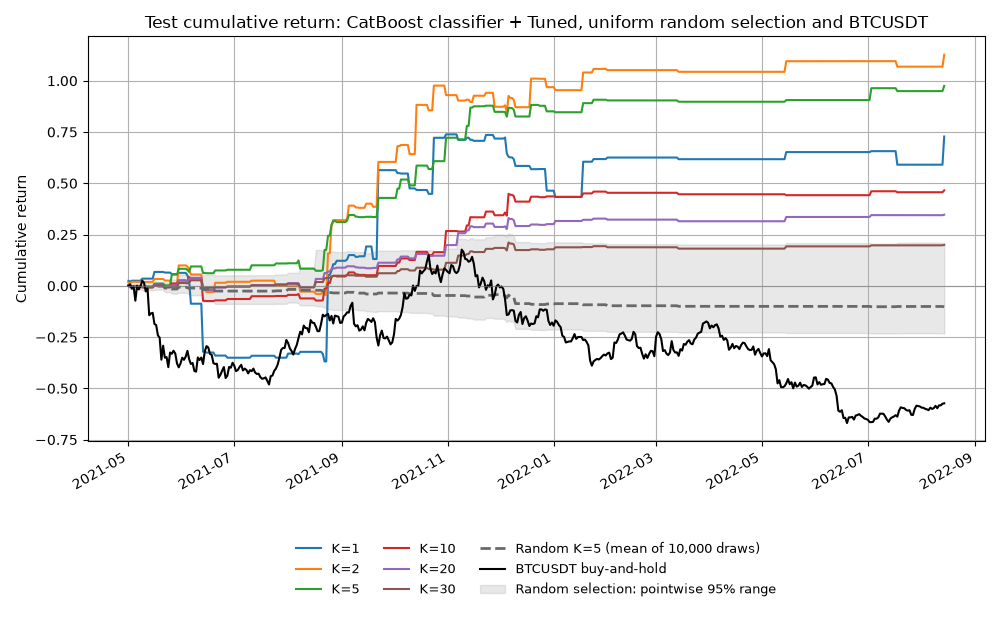
\includegraphics[width=\textwidth]{images/portfolios_vs_btc_test.png}
    \caption{CatBoost portfolio cumulative returns, random selection and BTC/USDT over the same calendar. Returns include 25 bp round-trip costs and exclude size-dependent impact. The dashed curve averages 10{,}000 random $k=5$ portfolios; shading is the pointwise 95\% selection range. The solid black line is BTC/USDT buy-and-hold.}
    \label{fig:portfolio_test}
\end{figure*}
BTC/USDT buy-and-hold has cumulative return $-0.573$, annualized return $-0.445$, annualized volatility $0.734$ and Sharpe $-0.606$. Its calendar runs from the first strategy decision to the last exit using completed one-minute conversion bars. BTC remains invested between events, whereas the model portfolios are exposed only during their event windows.

\subsection{Execution-Aware Backtesting with Price Impact}
\label{sec:price_impact}

The results above use the first observed trade at or after each execution threshold but do not otherwise charge size-dependent slippage, which is unrealistic for the illiquid small-cap tokens typically targeted by P\&D operations. To assess practical feasibility, we extend the backtesting framework with a fitted market-impact model that produces \emph{size-dependent, dynamic} slippage in addition to the fixed round-trip fee. The model serves two purposes: first, it estimates a volume-weighted average price (VWAP) for both entry and exit; second, the shape of the impact curve is itself the \emph{liquidity constraint} of the strategy---larger orders remain executable, but the fitted $\beta\sqrt{Q}$ curve makes each additional unit of notional arrive at progressively worse prices, so the economically relevant question shifts from ``is the order executable?'' to ``at what order size does impact erode the signal?''.

\subsubsection{Impact model specification}
We model price impact in basis points as a function of order notional $Q$ (in USDT):

\begin{equation}
    I(Q) = \beta \sqrt{Q}.
    \label{eq:impact_model}
\end{equation}

The square-root specification is a well-established empirical regularity in market microstructure. Kyle~\cite{kyle1985continuous} introduced the foundational model of linear price impact from informed order flow; subsequent work demonstrated that the aggregate impact of executed orders follows a concave, approximately square-root, relationship with order size. Almgren and Chriss~\cite{almgren2001optimal} formalized this within the optimal execution framework, while Almgren et al.~\cite{almgren2005direct} provided direct empirical estimates of the power-law exponent ($\approx 0.6$) using institutional equity data. Bouchaud et al.~\cite{bouchaud2009markets} surveyed the evidence for the square-root law across asset classes, and T\'{o}th et al.~\cite{toth2011anomalous} demonstrated its universality across stocks and time periods using a large meta-order dataset. In cryptocurrency markets specifically, Donier and Bonart~\cite{donier2015million} confirmed the square-root law in Bitcoin using over one million reconstructed meta-orders, showing that the relationship holds across four decades of order sizes.

We fit a single coefficient $\beta \geq 0$ via constrained OLS (no intercept) for each asset, pooling absolute impacts from both buy and sell candles. The entry regression uses the 14 days of 5-minute candles ending strictly at the actual simulated entry; it therefore cannot observe any later trade. For the manipulated asset, the execution backtest fits 5-second sell-dominated candles from $T$ up to, but excluding, the realized exit timestamp, capped at $T+10$ minutes. In each case, absolute net volume serves as $Q$ and the absolute close-to-close price change (in bps) serves as the impact observation. Entry notionals are converted to USDT using the most recent completed BTC/USDT one-minute bar at entry; the exit model uses the completed rate available at the announcement. Neither conversion falls forward to a future or incomplete bar.

\subsubsection{Impact measurement from candle data}
\textbf{Entry model (5-minute candles).} We aggregate the 14-day trade history ending strictly at the actual simulated entry timestamp into 5-minute candles. For each candle we compute the net buy volume $Q_{\mathrm{net}} = 2 \times V_{\mathrm{taker\,buy}} - V_{\mathrm{total}}$ (in quote currency), where $V_{\mathrm{taker\,buy}}$ is the taker-buy quote volume and $V_{\mathrm{total}}$ is the total quote volume. The absolute net volume $|Q_{\mathrm{net}}|$ serves as the order size, and the absolute close-to-close price change $|p_{\mathrm{close}} / p_{\mathrm{prev\,close}} - 1| \times 10^4$ bps serves as the impact observation. Observations from both buy- and sell-dominated candles are pooled into a single regression, which doubles the effective sample size and produces a more stable estimate of $\beta$. The 5-minute resolution matches the intended execution horizon: we assume the order is worked over a single candle interval, so the candle-level impact directly estimates the cost of execution.

\textbf{Exit model for manipulated assets (5-second candles, sell-only).} For the pumped asset, the backtest fits a separate model using only sell-dominated candles (negative $Q_{\mathrm{net}}$) in $[T,\min(T+10\mathrm{min},t_{\mathrm{exit}}))$. The right-open exit bound prevents post-exit observations from entering the simulated execution cost. The full 10-minute window is used only for the illustrative regression figure below.

We model liquidity through a continuous price-impact penalty rather than a hard participation cap. This makes larger orders executable only at increasingly adverse VWAPs. A hard order-book depth or participation-rate cap would further reduce realized returns and is therefore a conservative extension for future work.

\subsubsection{VWAP entry and exit price estimation}
\label{sec:vwap_estimation}

The execution simulation proceeds as follows for each selected asset:

\textbf{Step 1: Determine raw prices.} Once the model has scored the cross-section at $t_{\mathrm{pump}} - \Delta t_{\mathrm{buy}}$, the entry price $p^{\mathrm{entry}}$ is the first trade price at or after that decision timestamp and strictly before $t_{\mathrm{pump}}$. If no such trade occurs, the leg is not executable and is omitted. The exit price $p^{\mathrm{exit}}$ is the first trade price at or after $t_{\mathrm{pump}}$ (or $t_{\mathrm{pump}} + \Delta t_{\mathrm{sell}}$ for the manipulated asset). Thus no simulated fill predates the signal that generated it.

\textbf{Step 2: Resolve intended notional.} The target order size $Q_{\mathrm{intended}}$ is specified in USDT and converted to quote currency (BTC) using the indicative BTC/USDT rate at entry time. This normalization ensures that intended position sizes are comparable across BTC price regimes.

\textbf{Step 3: Track inventory and exit notional.} Let $R^{\mathrm{entry}}_{\mathrm{BTC/USDT}}$ denote the completed indicative conversion rate at entry. The entry quote notional and acquired base-asset quantity are
\begin{equation}
    Q^{\mathrm{entry}}_{\mathrm{BTC}}
      = Q_{\mathrm{intended}}/R^{\mathrm{entry}}_{\mathrm{BTC/USDT}},
    \qquad
    B = Q^{\mathrm{entry}}_{\mathrm{BTC}}/p^{\mathrm{entry}}_{\mathrm{vwap}}.
\end{equation}
The exit liquidates all $B$ units. Its impact is evaluated at the contemporaneous raw quote notional $Q^{\mathrm{exit}}_{\mathrm{BTC}}=B p^{\mathrm{exit}}$, rather than reusing the entry BTC notional. Internally the impact functions use USDT-normalized sizes $\widetilde Q^{\mathrm{entry}}=Q^{\mathrm{entry}}_{\mathrm{BTC}}R^{\mathrm{entry}}_{\mathrm{BTC/USDT}}$ and $\widetilde Q^{\mathrm{exit}}=Q^{\mathrm{exit}}_{\mathrm{BTC}}R^{T}_{\mathrm{BTC/USDT}}$, where $R^{T}$ is the completed announcement-time rate used to fit the manipulated exit model. This prevents exit slippage from being understated when the target price rises. We assume that deeper layers of the order book remain available beyond the volume observed in historical candles. Larger trades therefore remain feasible, but they incur larger slippage through the impact model.

\textbf{Step 4: Compute VWAP execution prices.} The fitted coefficient estimates the price displacement associated with a given net order flow. An order that walks through the book continuously fills at improving prices along the way. Integrating the square-root impact profile over the execution path yields the average fill cost:
\begin{equation}
    I_{\mathrm{vwap}}(Q)
      = \frac{1}{Q}\int_{0}^{Q}\!\beta\sqrt{v}\,dv
      = \tfrac{2}{3}\,\beta\sqrt{Q}.
    \label{eq:vwap_correction}
\end{equation}
The VWAP impact is two-thirds of the terminal impact because early fills occur at better prices than the final fill level. The VWAP execution prices are then:
\begin{align}
    p^{\mathrm{entry}}_{\mathrm{vwap}} &= p^{\mathrm{entry}}\;\bigl(1 + I_{\mathrm{vwap}}(\widetilde Q^{\mathrm{entry}}) / 10^4\bigr), \label{eq:vwap_entry}\\
    p^{\mathrm{exit}}_{\mathrm{vwap}}  &= p^{\mathrm{exit}}\;\bigl(1 - I_{\mathrm{vwap}}(\widetilde Q^{\mathrm{exit}}) / 10^4\bigr). \label{eq:vwap_exit}
\end{align}
Buying pushes the fill price above the initial quote; selling pushes it below. Let $R^{\mathrm{exit}}_{\mathrm{BTC/USDT}}$ be the completed exit-time conversion rate. The fully USDT-denominated transaction return is
\begin{equation}
    r_{\mathrm{USDT}}
      = \frac{B p^{\mathrm{exit}}_{\mathrm{vwap}} R^{\mathrm{exit}}_{\mathrm{BTC/USDT}}}
             {Q_{\mathrm{intended}}}
        - 1 - 0.0025,
    \label{eq:tx_return}
\end{equation}
where the 25 bps term is charged against entry capital and covers the round-trip exchange fee. This accounting includes the BTC/USDT move over the holding interval and never mixes a BTC-denominated asset return with an exit-time USDT conversion.

\textbf{Manipulated-asset exit.} The sell leg occurs during the manipulation window where buying and selling pressure are not balanced. Its impact model uses 5-second sell-dominated candles available strictly before the exit, never observations after the simulated transaction. A manipulation-window fit is used only when at least 20 sell-dominated candle samples are available; otherwise the framework falls back to the pre-pump entry model. The ten-minute diagnostic fit below is illustrative; each execution fit uses only observations before its own exit.

\subsubsection{Regression fit quality}
Fig.~\ref{fig:impact_regression} shows an example of the fitted entry impact regression for one pump asset. The absolute-impact approach pools buy and sell 5-minute candles into a single regression ($I = \beta\sqrt{Q}$, no intercept), yielding $R^2 = 0.310$ on the buy side, $R^2 = 0.355$ on the sell side, and $\beta = 0.7224$ in the example shown.

Fig.~\ref{fig:exit_impact_regression} is a descriptive fit over the full capped 10-minute manipulation window for one asset. This longer diagnostic window is used only to visualize the sell-side relation; the execution backtest instead truncates each fit at that transaction's realized exit. The sell-only 5-second candle approach yields $R^2 = 0.274$ with $\beta = 1.3188$ ($n = 83$ candles) in the example shown. These illustrative coefficients do not establish a general causal difference between entry and exit liquidity.

\begin{figure*}[!t]
    \centering
    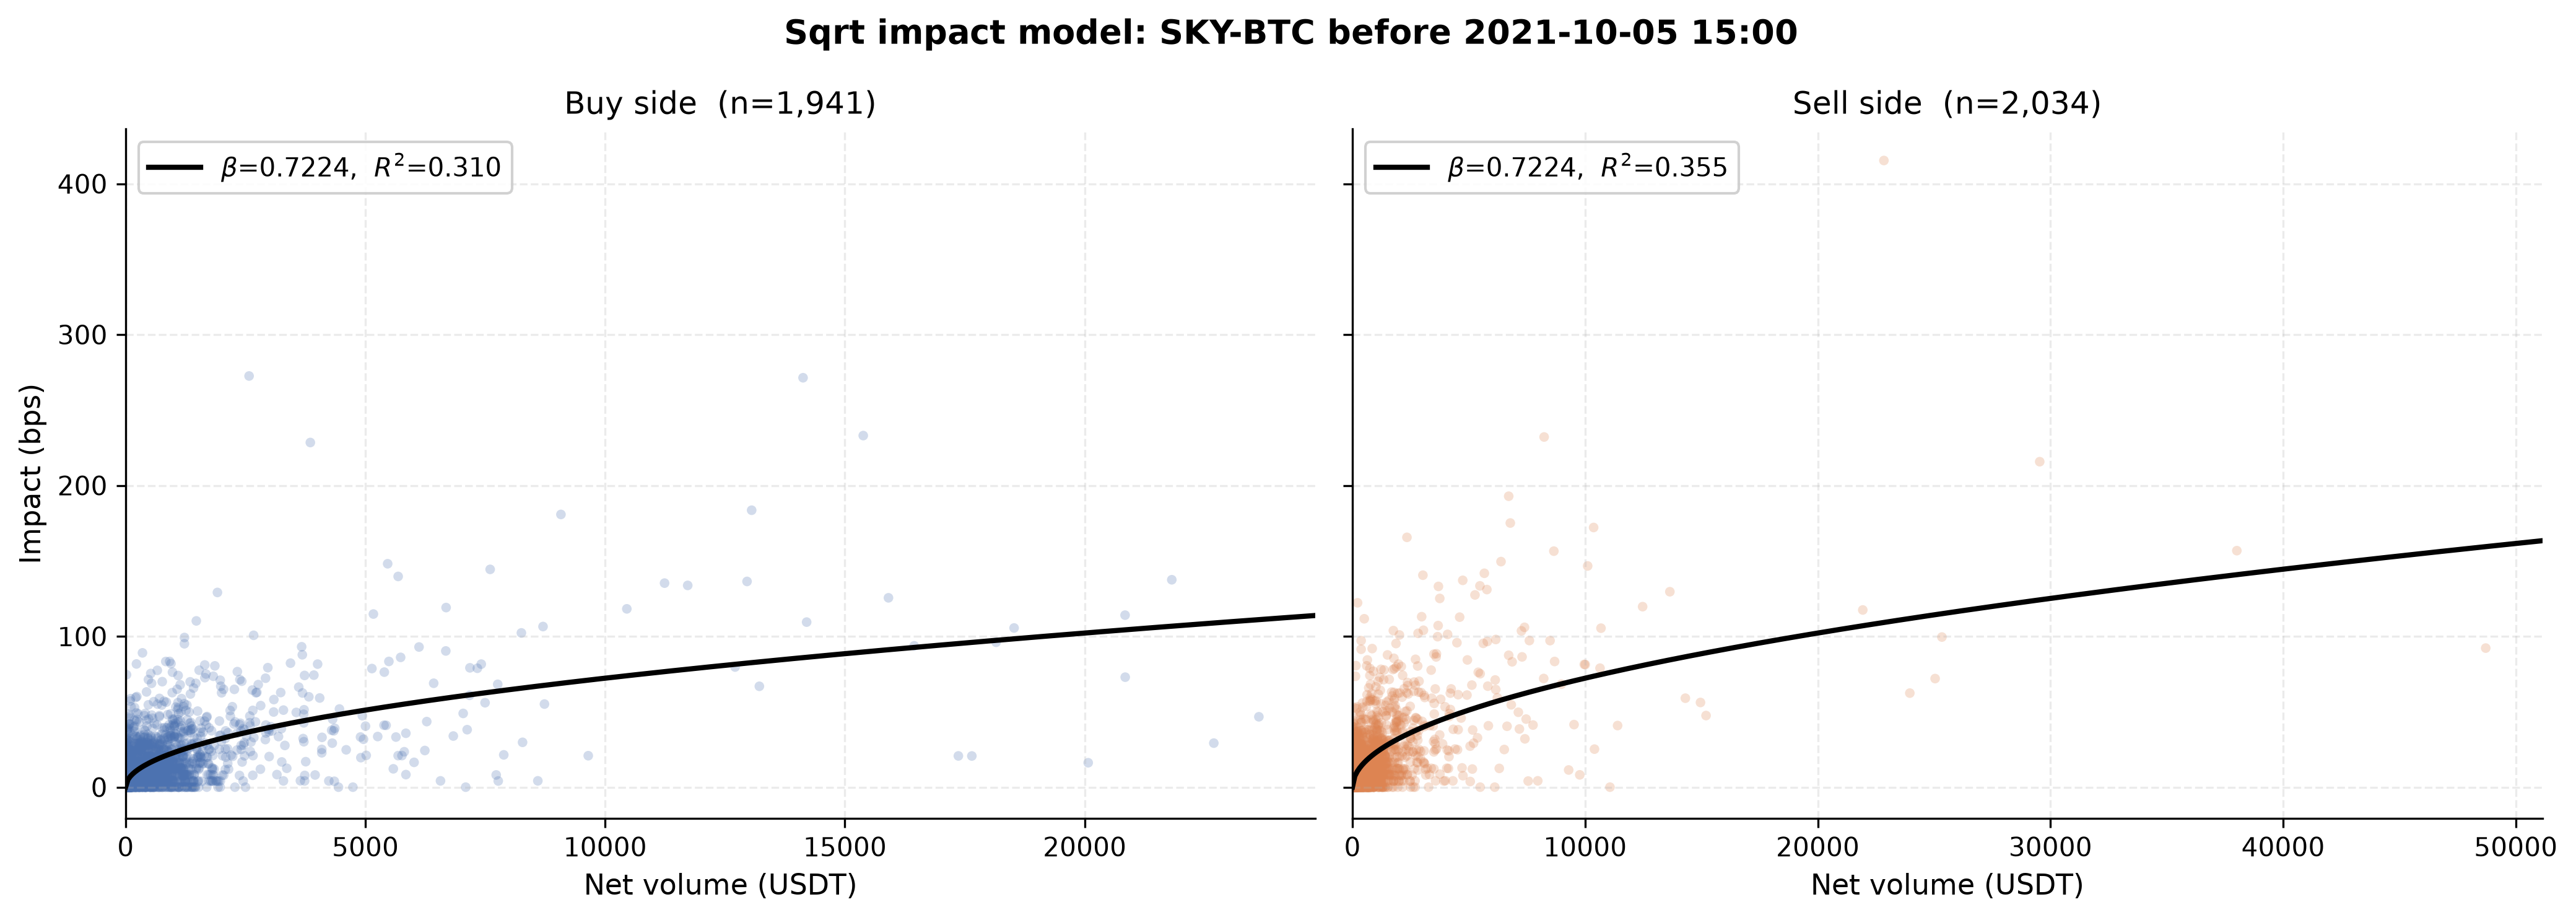
\includegraphics[width=\textwidth]{images/impact_regression_example.png}
    \caption{Fitted entry price-impact regression for the SKY-BTC pair, using the 14 trading days of 5-minute candles ending 15 minutes before the pump announcement. Left panel: candles with net buying pressure (positive $Q_{\mathrm{net}}$); right panel: candles with net selling pressure (negative $Q_{\mathrm{net}}$). Each scatter point is one 5-minute candle; horizontal axis $|Q_{\mathrm{net}}|$ is absolute net volume in USDT and vertical axis $|\Delta p|$ is the absolute close-to-close price change in basis points. Solid line: fitted $|\Delta p| = \beta\sqrt{|Q_{\mathrm{net}}|}$ (no intercept, $\beta = 0.72$), estimated on both panels jointly. \textbf{Takeaway:} the single-parameter square-root fit captures the concave impact$-$size relation on both sides of the book, consistent with the square-root impact law documented across asset classes~\cite{toth2011anomalous,donier2015million}; this is the curve used to translate order size into VWAP slippage in the backtest.}
    \label{fig:impact_regression}
\end{figure*}

\begin{figure}[!t]
    \centering
    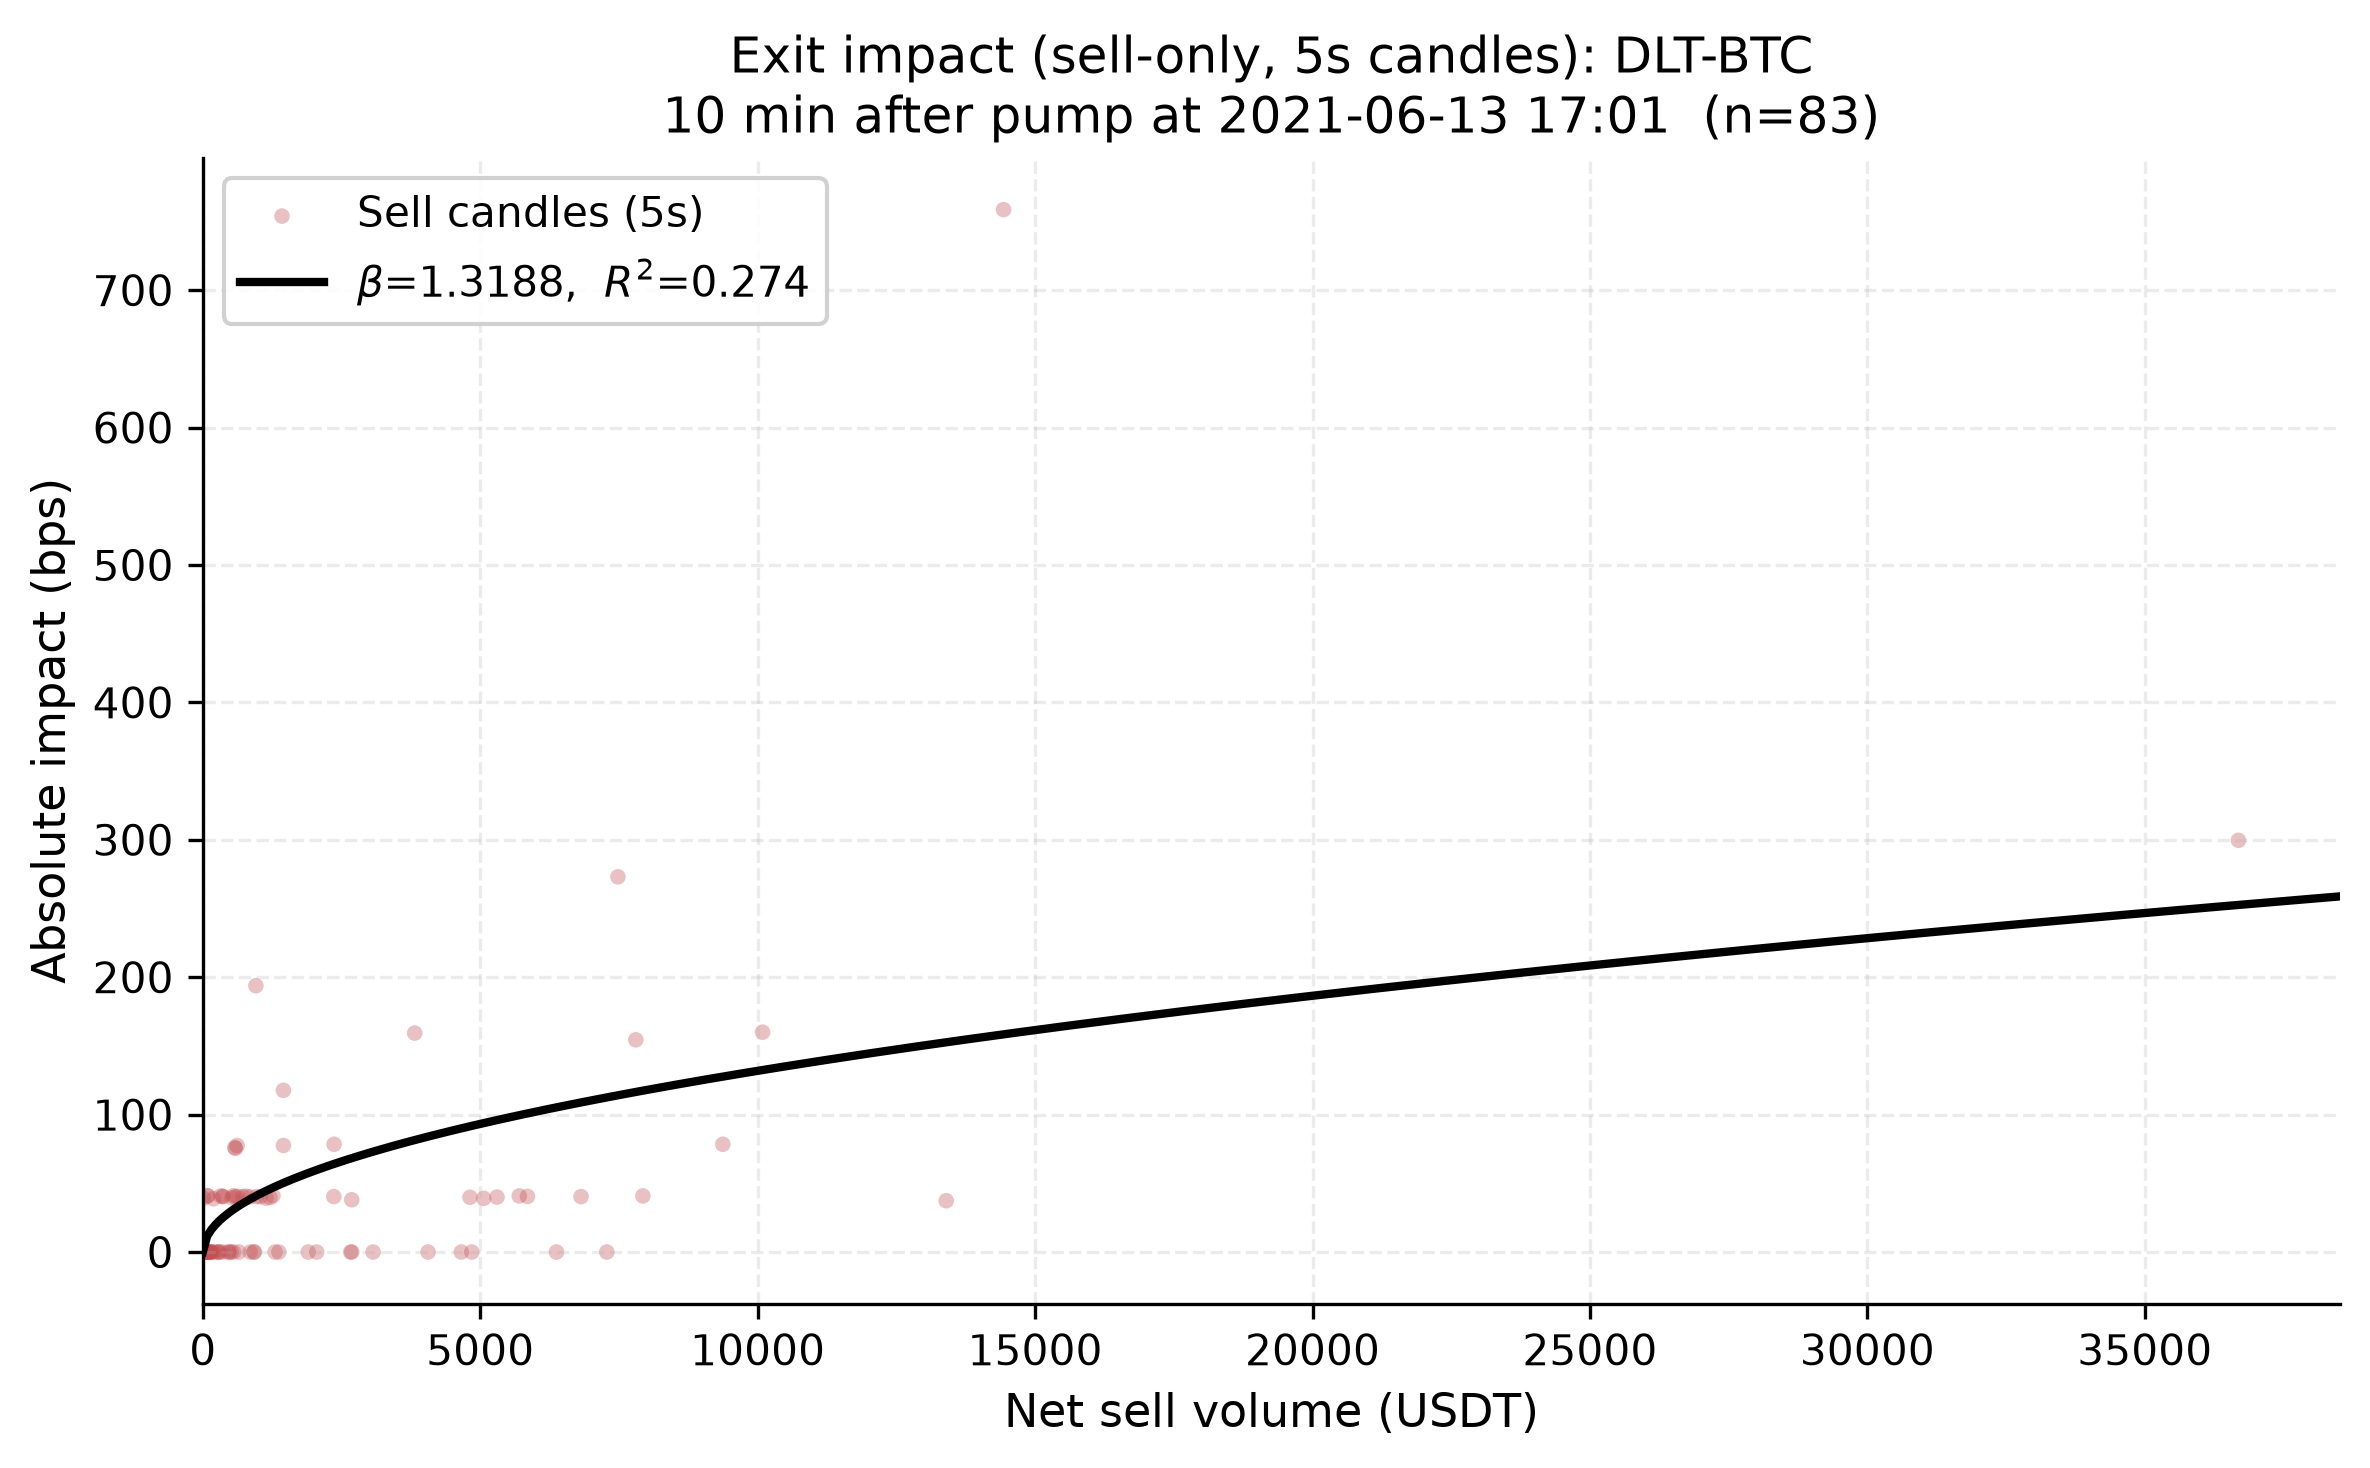
\includegraphics[width=\columnwidth]{images/exit_impact_regression_example.png}
    \caption{Descriptive exit price-impact regression for the DLT-BTC pair, using 5-second candles from the first 10 minutes after the pump announcement and restricted to sell-dominated candles ($n = 83$). This full-window illustration is not the execution fit: each backtested exit uses only candles strictly preceding its own exit timestamp. Horizontal axis: absolute sell-side net notional $|Q_{\mathrm{net}}|$ in USDT. Vertical axis: absolute close-to-close price change in basis points. Solid line: fitted $|\Delta p| = \beta\sqrt{|Q_{\mathrm{net}}|}$ ($\beta = 1.32$). \textbf{Takeaway:} the exit coefficient is nearly twice the entry coefficient ($1.32$ vs.\ $0.72$ on the earlier example), which illustrates different fitted coefficients in these two examples rather than a general estimate of the relative cost of entry and exit.}
    \label{fig:exit_impact_regression}
\end{figure}

\subsubsection{Unmodeled execution frictions}
The fitted impact model captures average slippage against historical candle-level liquidity but intentionally omits several real-world frictions in order to keep the estimate interpretable. Specifically, we do not model (i) order-book depth exhaustion at the deepest levels (which would manifest as partial fills rather than a smooth $\beta\sqrt{Q}$ curve), (ii) queue priority and time-in-force dynamics on the exchange matching engine, (iii) exchange-side API latency between signal generation and order arrival, and (iv) the risk that other market participants detect the same pump signature and front-run the entry. Each of these frictions works in the same direction and would reduce realized PnL further, so the sensitivity numbers reported below should be read as assumption-dependent scenarios, not a validated upper bound on achievable performance.

\subsubsection{Portfolio performance with price impact}
We apply the fitted impact model to both execution legs with 1{,}000 USDT per selected asset, so a size-$k$ portfolio targets $k\times1{,}000$ USDT per event. Predictions, event order, random selections and other trading rules are identical to the no-impact comparison. At $k=5$, CatBoost cumulative return is $61.49\%$ and Sharpe is $1.87$. Random selection has mean return $-32.99\%$, with a central 95\% range of $[-46.11\%,\,-2.22\%]$.
\begin{table*}[!t]
    \centering
    \small
    \setlength{\tabcolsep}{5pt}
    \renewcommand{\arraystretch}{1.15}
    \caption{Portfolio performance with 1{,}000 USDT per asset, fitted entry and exit impact, and 25 bp costs. Random rows average 10{,}000 draws; returns are decimal fractions.}
    \resizebox{\ifdim\width>\textwidth\textwidth\else\width\fi}{!}{%
    \begin{tabular}{lrrrrr}
        \toprule
        Portfolio & Avg. event return & Cumulative return & Annualized return & Annualized volatility & Sharpe \\
        \midrule
        CatBoost $k=1$ & 0.0044 & 0.3496 & 0.2709 & 0.6806 & 0.3980 \\
        CatBoost $k=2$ & 0.0093 & 0.7467 & 0.5787 & 0.4468 & 1.2951 \\
        CatBoost $k=5$ & 0.0077 & 0.6149 & 0.4766 & 0.2549 & 1.8693 \\
        CatBoost $k=10$ & 0.0014 & 0.1113 & 0.0863 & 0.2026 & 0.4259 \\
        CatBoost $k=20$ & 0.0001 & 0.0048 & 0.0037 & 0.1289 & 0.0291 \\
        CatBoost $k=30$ & -0.0016 & -0.1298 & -0.1006 & 0.0904 & -1.1131 \\
        Random $k=1$ & -0.0041 & -0.3300 & -0.2557 & 0.1394 & -2.8156 \\
        Random $k=2$ & -0.0041 & -0.3293 & -0.2552 & 0.1174 & -3.1083 \\
        Random $k=5$ & -0.0041 & -0.3299 & -0.2556 & 0.0932 & -3.3821 \\
        Random $k=10$ & -0.0041 & -0.3307 & -0.2562 & 0.0792 & -3.6087 \\
        Random $k=20$ & -0.0041 & -0.3311 & -0.2566 & 0.0687 & -3.8887 \\
        Random $k=30$ & -0.0041 & -0.3313 & -0.2567 & 0.0641 & -4.0733 \\
        BTCUSDT buy-and-hold & --- & -0.5727 & -0.4448 & 0.7340 & -0.6060 \\
        \bottomrule
    \end{tabular}
    }
    \label{table:performance_by_k_impact}
\end{table*}
\begin{figure*}[!t]
    \centering
    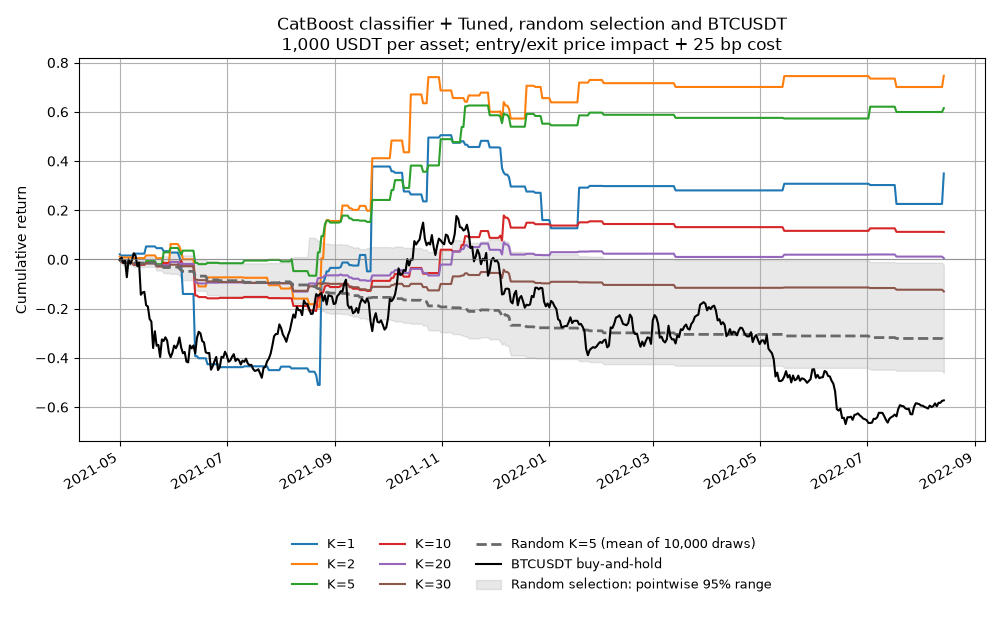
\includegraphics[width=\textwidth]{images/portfolios_1000usdt_with_slippage.png}
    \caption{The same portfolios and random selections as Fig.~\ref{fig:portfolio_test}, with fitted price impact on both legs at 1{,}000 USDT per asset. Shading is the pointwise 95\% random-selection range; the BTC/USDT benchmark is unchanged.}
    \label{fig:portfolio_test_impact}
\end{figure*}
\subsubsection{PnL sensitivity to order size}
For $k=5$, we vary intended size from 100 to 10{,}000 USDT per asset. Cumulative ROE without reinvestment is $0.861$ at 100 USDT, $0.467$ at 2{,}000 USDT, $0.174$ at 5{,}000 USDT, and $-0.155$ at 10{,}000 USDT. These conditional simulation outcomes depend on fill and impact assumptions and do not establish executable capacity.
\begin{figure}[!t]
    \centering
    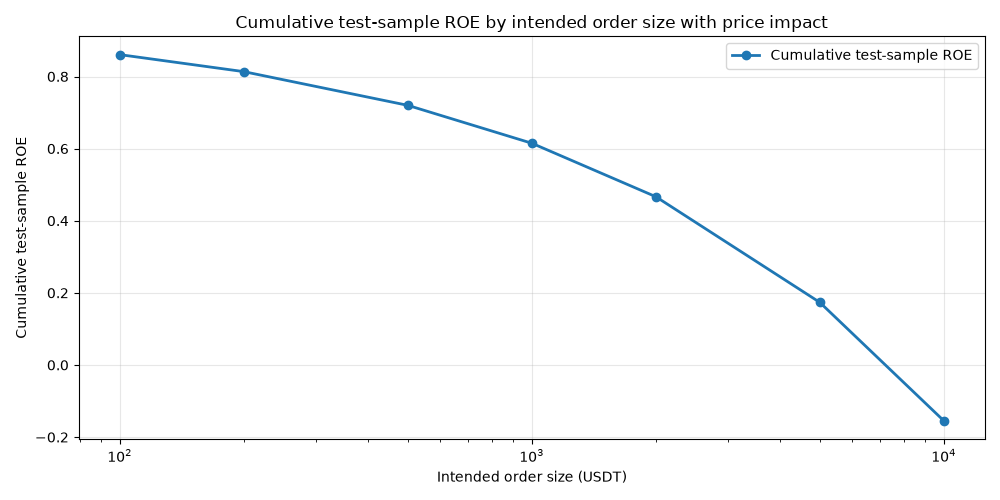
\includegraphics[width=\columnwidth]{images/pnl_vs_quantity_with_impact.png}
    \caption{CatBoost cumulative ROE over the 80 test events as intended per-asset notional changes. The $k=5$ strategy includes fitted entry and exit impact and 25 bp costs; returns are summed without reinvestment.}
    \label{fig:pnl_vs_quantity}
\end{figure}

\section{Limitations and Future Work}
\label{sec:limitations}

\textbf{Exchange generalizability.}
Our analysis is restricted to Binance BTC pairs during 2018--2022. The evidence does not establish generalisation to USDT pairs, other exchanges, decentralised venues, later market regimes, or continuous surveillance when announcement times are unknown. Each extension requires new labels, point-in-time features, and out-of-period or external validation.

\textbf{Dataset size.}
With 473 analyzed events (80 in test), statistical power remains limited. The reported intervals condition on the fitted models and assume independent pump events; correlated campaigns and test-set reuse may make them optimistic. The paired comparison in Section~\ref{sec:significance} does not establish a statistically significant AUC advantage for CatBoost + ES over tuned CatBoost.
\textbf{Execution assumptions.}
The fitted impact and 25 bp cost assumptions do not establish real trading feasibility. Order-book depth, queue priority, partial fills, signal/API latency, front-running, and exchange access restrictions are incompletely observed. Historical transaction prices do not guarantee executable quotes or scalable capacity. Predictive hit rates and simulated PnL are therefore separate outcomes, and positive simulated returns are not evidence of attainable live profits.

\textbf{Evolving manipulation tactics.}
Manipulators may adapt their strategies over time. The late test subperiod has too few events for a reliable comparison, so our subperiod analysis does not establish cross-regime stability. Later chronological holdouts and monitoring would be needed for deployment.

\textbf{Alternative imbalance-handling approaches.}
While we compared class weighting and SMOTE, other techniques such as focal loss~\cite{lin2017focal}, cost-sensitive learning~\cite{elkan2001cost}, and deep anomaly detection~\cite{liu2008isolation} remain unexplored in this setting and could potentially improve performance.

\textbf{Temporal safeguards and reproducibility.}
The pipeline uses only data available before each decision. Feature windows and normalization data end strictly before $T-15$ minutes, and missing-value estimates are learned only from the training set. Automated tests add future trades, listings, and pump announcements to confirm that eligible assets and features do not change. They also check timestamp boundaries, exclude outcome variables from model inputs, keep test data out of training and tuning, and verify that currency conversion uses completed bars and price-impact estimates exclude trades after execution. These tests found no use of future data in the cases checked.

The repository provides the event cohort, split membership, software versions, seed settings, feature hashes, model parameters, test predictions, shared bootstrap draws, and random-portfolio selections and execution outcomes. The same saved predictions underlie the test comparison, resampling and portfolios. The event records cannot independently validate Telegram annotations because the underlying messages and URLs are unavailable.


\section{Conclusion}

This study compares seven tuned imbalance-aware prediction models on the same Binance BTC-pair events. Validation selects CatBoost (Top@k\%AUC $0.653$), which achieves test AUC $0.689$ and Top@5 $0.450$. L2 logistic regression has the largest descriptive test AUC ($0.710$), but paired resampling does not establish its superiority over CatBoost. The same selected model supplies all portfolio analyses: its $k=5$ cumulative return is $97.46\%$ without size-dependent impact and $61.49\%$ with fitted impact at 1{,}000 USDT per asset. These simulation outcomes are sensitive to execution assumptions and order size.

The evaluated SMOTE and ranking variants are weaker than the leading classifiers in this sample. These results motivate further work on market surveillance, with independent label verification and external chronological validation needed before broader claims or operational use.


\begin{thebibliography}{00}

\bibitem{optuna_2019} T.~Akiba, S.~Sano, T.~Yanase, T.~Ohta, and M.~Koyama, ``Optuna: A next-generation hyperparameter optimization framework,'' in \emph{Proc. 25th ACM SIGKDD Int. Conf. Knowl. Discovery Data Mining}, 2019.

\bibitem{albers_frag_2022} J.~Albers, M.~Cucuringu, S.~Howison, and A.~Y.~Shestopaloff, ``Fragmentation, price formation and cross-impact in Bitcoin markets,'' \emph{Appl. Math. Finance}, vol.~28, 2022.

\bibitem{random_forest_2001} L.~Breiman, ``Random forests,'' \emph{Mach. Learn.}, vol.~45, no.~1, 2001.

\bibitem{chadalapaka_crypto_2022} V.~Chadalapaka, K.~Chang, G.~Mahajan, and A.~Vasil, ``Crypto pump and dump detection via deep learning techniques,'' \emph{arXiv}, 2022.

\bibitem{cong_washtrading_2023} L.~W.~Cong, X.~Li, K.~Tang, and Y.~Yang, ``Crypto wash trading,'' \emph{Manage. Sci.}, vol.~69, no.~11, 2023.

\bibitem{econometrics11030022} D.~Fantazzini and Y.~Xiao, ``Detecting pump-and-dumps with crypto-assets: Dealing with imbalanced datasets and insiders' anticipated purchases,'' \emph{Econometrics}, vol.~11, no.~3, 2023.

\bibitem{grinsztajn_2022} L.~Grinsztajn, O.~Oyallon, and G.~Varoquaux, ``Why do tree-based models still outperform deep learning on typical tabular data?,'' in \emph{Advances in Neural Information Processing Systems}, 2022.

\bibitem{hu2023sequence} S.~Hu, Z.~Zhang, S.~Lu, B.~He, and Z.~Li, ``Sequence-based target coin prediction for cryptocurrency pump-and-dump,'' \emph{Proc. ACM Manag. Data}, vol.~1, no.~1, 2023.

\bibitem{kamps_moon_2018} J.~Kamps and K.~Bennett, ``To the moon: Defining and detecting cryptocurrency pump-and-dumps,'' \emph{Crime Sci.}, vol.~7, p.~18, 2018.

\bibitem{la_morgia_pump_2020} M.~La~Morgia, A.~Mei, F.~Sassi, and J.~Stefa, ``Pump and dumps in the Bitcoin era: Real-time detection of cryptocurrency market manipulations,'' in \emph{Proc. Int. Conf. Comput. Commun. Netw. (ICCCN)}, 2020, pp.~1--9.

\bibitem{la2023doge} M.~La~Morgia, A.~Mei, F.~Sassi, and J.~Stefa, ``The doge of wall street: Analysis and detection of pump-and-dump cryptocurrency manipulations,'' \emph{ACM Trans. Internet Technol.}, vol.~23, no.~1, pp.~1--28, 2023.

\bibitem{nghiem_2021} H.~Nghiem, G.~Muric, F.~Morstatter, and E.~Ferrara, ``Detecting cryptocurrency pump-and-dump frauds using market and social signals,'' \emph{Expert Syst. Appl.}, art. no. 115284, 2021.

\bibitem{ntakaris_midprice_2022} A.~Ntakaris, J.~Kanniainen, M.~Gabbouj, and A.~Iosifidis, ``Mid-price prediction based on machine learning methods with technical and quantitative indicators,'' \emph{PLOS ONE}, vol.~15, no.~6, 2020.

\bibitem{poh_ltr} D.~Poh, B.~Lim, S.~Zohren, and S.~Roberts, ``Building cross-sectional systematic strategies by learning to rank,'' \emph{J. Financial Data Sci.}, vol.~3, no.~2, pp.~70--86, 2021.

\bibitem{catboost} L.~Prokhorenkova, G.~Gusev, A.~Vorobev, A.~V.~Dorogush, and A.~Gulin, ``CatBoost: Unbiased boosting with categorical features,'' in \emph{Advances in Neural Information Processing Systems}, 2018.

\bibitem{pd_anatomy} J.~Xu and B.~Livshits, ``The anatomy of a cryptocurrency pump-and-dump scheme,'' in \emph{Proc. 28th USENIX Secur. Symp. (USENIX Security 19)}, 2019, pp.~1609--1625.

\bibitem{chawla2002smote} N.~V.~Chawla, K.~W.~Bowyer, L.~O.~Hall, and W.~P.~Kegelmeyer, ``SMOTE: Synthetic minority over-sampling technique,'' \emph{J. Artif. Intell. Res.}, vol.~16, pp.~321--357, 2002.

\bibitem{code_github}
M.~Mironov, D.~Bogutsky, and P.~Lukianchenko, ``Pump-and-dump target prediction (code repository), GitHub, 2025. [Online]. Available: https://github.com/B0R0koko/pump-and-dump-prediction. Accessed on: Nov.~2,~2026.


\bibitem{almgren2001optimal} R.~Almgren and N.~Chriss, ``Optimal execution of portfolio transactions,'' \emph{J. Risk}, vol.~3, no.~2, pp.~5--39, 2001.

\bibitem{almgren2005direct} R.~Almgren, C.~Thum, E.~Hauptmann, and H.~Li, ``Direct estimation of equity market impact,'' \emph{Risk}, vol.~18, no.~7, pp.~58--62, 2005.

\bibitem{blagus2013smote} R.~Blagus and L.~Lusa, ``SMOTE for high-dimensional class-imbalanced data,'' \emph{BMC Bioinform.}, vol.~14, p.~106, 2013.

\bibitem{bouchaud2009markets} J.-P.~Bouchaud, J.~D.~Farmer, and F.~Lillo, ``How markets slowly digest changes in supply and demand,'' in \emph{Handbook of Financial Markets: Dynamics and Evolution}, T.~Hens and K.~R.~Schenk-Hopp\'{e}, Eds.\hspace{0.25em} Elsevier, 2009, ch.~2.

\bibitem{donier2015million} J.~Donier and J.~Bonart, ``A million metaorder analysis of market impact on the Bitcoin,'' \emph{Market Microstructure and Liquidity}, vol.~1, no.~2, art.~1550008, 2015.

\bibitem{elkan2001cost} C.~Elkan, ``The foundations of cost-sensitive learning,'' in \emph{Proc. 17th Int. Joint Conf. Artif. Intell. (IJCAI)}, 2001, pp.~973--978.

\bibitem{kyle1985continuous} A.~S.~Kyle, ``Continuous auctions and insider trading,'' \emph{Econometrica}, vol.~53, no.~6, pp.~1315--1335, 1985.

\bibitem{lin2017focal} T.-Y.~Lin, P.~Goyal, R.~Girshick, K.~He, and P.~Doll\'{a}r, ``Focal loss for dense object detection,'' in \emph{Proc. IEEE Int. Conf. Comput. Vis. (ICCV)}, 2017, pp.~2980--2988.

\bibitem{liu2008isolation} F.~T.~Liu, K.~M.~Ting, and Z.-H.~Zhou, ``Isolation forest,'' in \emph{Proc. IEEE Int. Conf. Data Mining (ICDM)}, 2008, pp.~413--422.

\bibitem{toth2011anomalous} B.~T\'{o}th, Y.~Lemperiere, C.~Deremble, J.~de~Lataillade, J.~Kockelkoren, and J.-P.~Bouchaud, ``Anomalous price impact and the critical nature of liquidity in financial markets,'' \emph{Phys. Rev. X}, vol.~1, art.~021006, 2011.


\bibitem{kapoor2023leakage} S.~Kapoor and A.~Narayanan, ``Leakage and the reproducibility crisis in machine-learning-based science,'' \emph{Patterns}, vol.~4, no.~9, art.~100804, 2023, doi: 10.1016/j.patter.2023.100804.

\bibitem{cerqueira2020evaluation} V.~Cerqueira, L.~Torgo, and I.~Mozeti\v{c}, ``Evaluating time series forecasting models: An empirical study on performance estimation methods,'' \emph{Mach. Learn.}, vol.~109, pp.~1997--2028, 2020, doi: 10.1007/s10994-020-05910-7.

\bibitem{chen2024imbalance} W.~Chen, K.~Yang, Z.~Yu, Y.~Shi, and C.~L.~P.~Chen, ``A survey on imbalanced learning: Latest research, applications and future directions,'' \emph{Artif. Intell. Rev.}, vol.~57, art.~137, 2024, doi: 10.1007/s10462-024-10759-6.

\bibitem{galati2024fees} L.~Galati, ``Exchange market share, market makers, and murky behavior: The impact of no-fee trading on cryptocurrency market quality,'' \emph{J. Banking Finance}, art.~107222, 2024, doi: 10.1016/j.jbankfin.2024.107222.

\end{thebibliography}

\begin{IEEEbiography}[{
\includegraphics[width=1in,height=1.25in,clip,keepaspectratio]{images/mironov.png}}]{Mikhail Mironov}
received the B.S.\ degree in economics from Universitat Pompeu Fabra, Barcelona, Spain, and the National Research University Higher School of Economics (HSE), St.\ Petersburg, Russia, in 2023 (double degree), and the M.S.\ degree with honors in financial economics from International College of Economics and Finance, ICEF HSE, Moscow, Russia, in 2025. He is currently pursuing the Ph.D.\ degree in finance at HSE, Moscow, Russia. His major field of study is finance and financial economics.

\end{IEEEbiography}

\begin{IEEEbiography}[{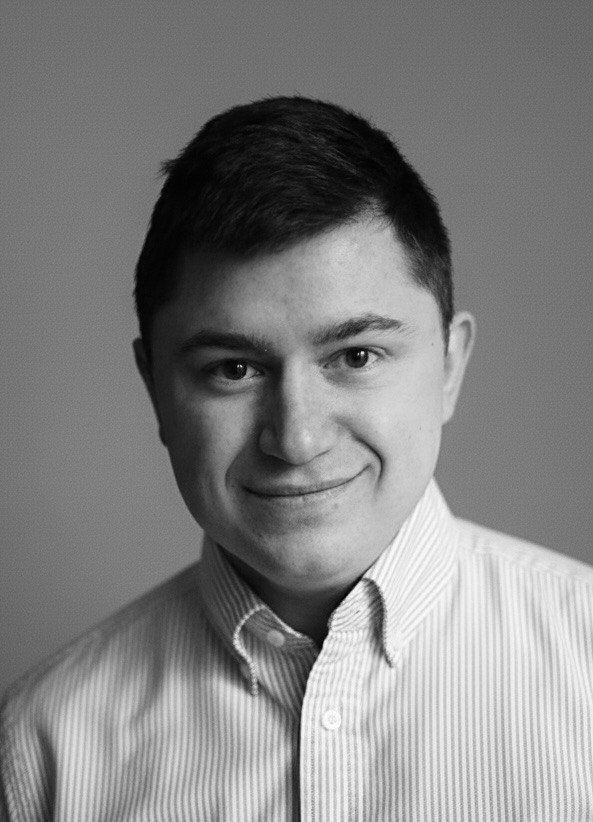
\includegraphics[width=1in,height=1.25in,clip,keepaspectratio]{images/bogutsky.png}}]{Denis Bogutsky} received the M.S. degree in mathematics from Lomonosov Moscow State University in 2020. He is currently a Junior Researcher with the Laboratory of AI in Mathematical Finance at the National Research University Higher School of Economics. His research focuses on quantitative finance, market microstructure, credit risk modeling, and anomaly detection in financial systems.
\end{IEEEbiography}

\newpage

%If you do not have or do not want to include a photo, you can use IEEEbiographynophoto as shown below:

\begin{IEEEbiography}
[{
\includegraphics[width=1in,height=1.25in,clip,keepaspectratio]{images/lukyanchenko.png}}]
{PETR P. LUKIANCHENKO} received the bachelor’s and master’s degrees in information science from HSE University, Moscow, Russia, in
2009 and 2011, respectively, and the Ph.D. degree
in mathematics. He has been with HSE University,
since 2009.
He currently holds multiple positions, including
a Senior Lecturer with the Faculty of Computer
Science, Big Data and Information Retrieval
School; a Lecturer with the Centre for Training
Top AI Professionals; and the Head of the Laboratory of Artificial Intelligence in Mathematical Finance, AI and Digital Science Institute. At Trusted
AI Research Center, he conducts research projects with a particular focus
on image processing and time series data. He has co-authored research on
neural-network-based approaches for predicting anomalies in interest rates
under stochastic noise. He has presented his work on a multiagent simulator
for financial crisis modeling at AI Journey 2025 Conference. His research
interests include artificial intelligence applications in finance, including the
detection of structural breaks in financial time series and the development of
simulators for financial market crises.

\end{IEEEbiography}

\EOD

\end{document}
